\documentclass[11pt]{article}
\usepackage[textwidth=18.0cm, textheight=23.0cm, top=2.0cm]{geometry}
\usepackage{pst-all}
\usepackage{amssymb}
\usepackage{tikz}
\usepackage{underscore}\begin{document}
\pagestyle{empty}


ClassName: \underline{\textbf{Class_08.2bp-45}}
\par
BinSize: \underline{\textbf{100 × 100}}
\par
ReduceSize: \underline{\textbf{100 × 100}}
\par
TypeNum: \underline{\textbf{99}}
\par
Num: \underline{\textbf{100}}
\par
OutS: \underline{\textbf{270000}}
\par
InS: \underline{\textbf{225982}}
\par
Rate: \underline{\textbf{0.837}}
\par
UB: \underline{\textbf{27}}
\par
LB0: \underline{\textbf{26}}
\par
LB: \underline{\textbf{27}}
\par
LBWithCut: \underline{\textbf{27}}
\par
NodeCut: \underline{\textbf{0}}
\par
ExtendedNodeCnt: \underline{\textbf{1}}
\par
GenNodeCnt: \underline{\textbf{1}}
\par
PrimalNode: \underline{\textbf{0}}
\par
ColumnCount: \underline{\textbf{267}}
\par
TotalCutCount: \underline{\textbf{0}}
\par
RootCutCount: \underline{\textbf{0}}
\par
LPSolverCnt: \underline{\textbf{241}}
\par
PricingSolverCnt: \underline{\textbf{241}}
\par
BranchAndBoundNum: \underline{\textbf{1}}
\par
isOpt: \underline{\textbf{true}}
\par
TimeOnPrimal: \underline{\textbf{0.000 s}}
\par
TimeOnPricing: \underline{\textbf{23.409 s}}
\par
TimeOnRmp: \underline{\textbf{0.205 s}}
\par
TotalTime: \underline{\textbf{23.754 s}}
\par
\newpage


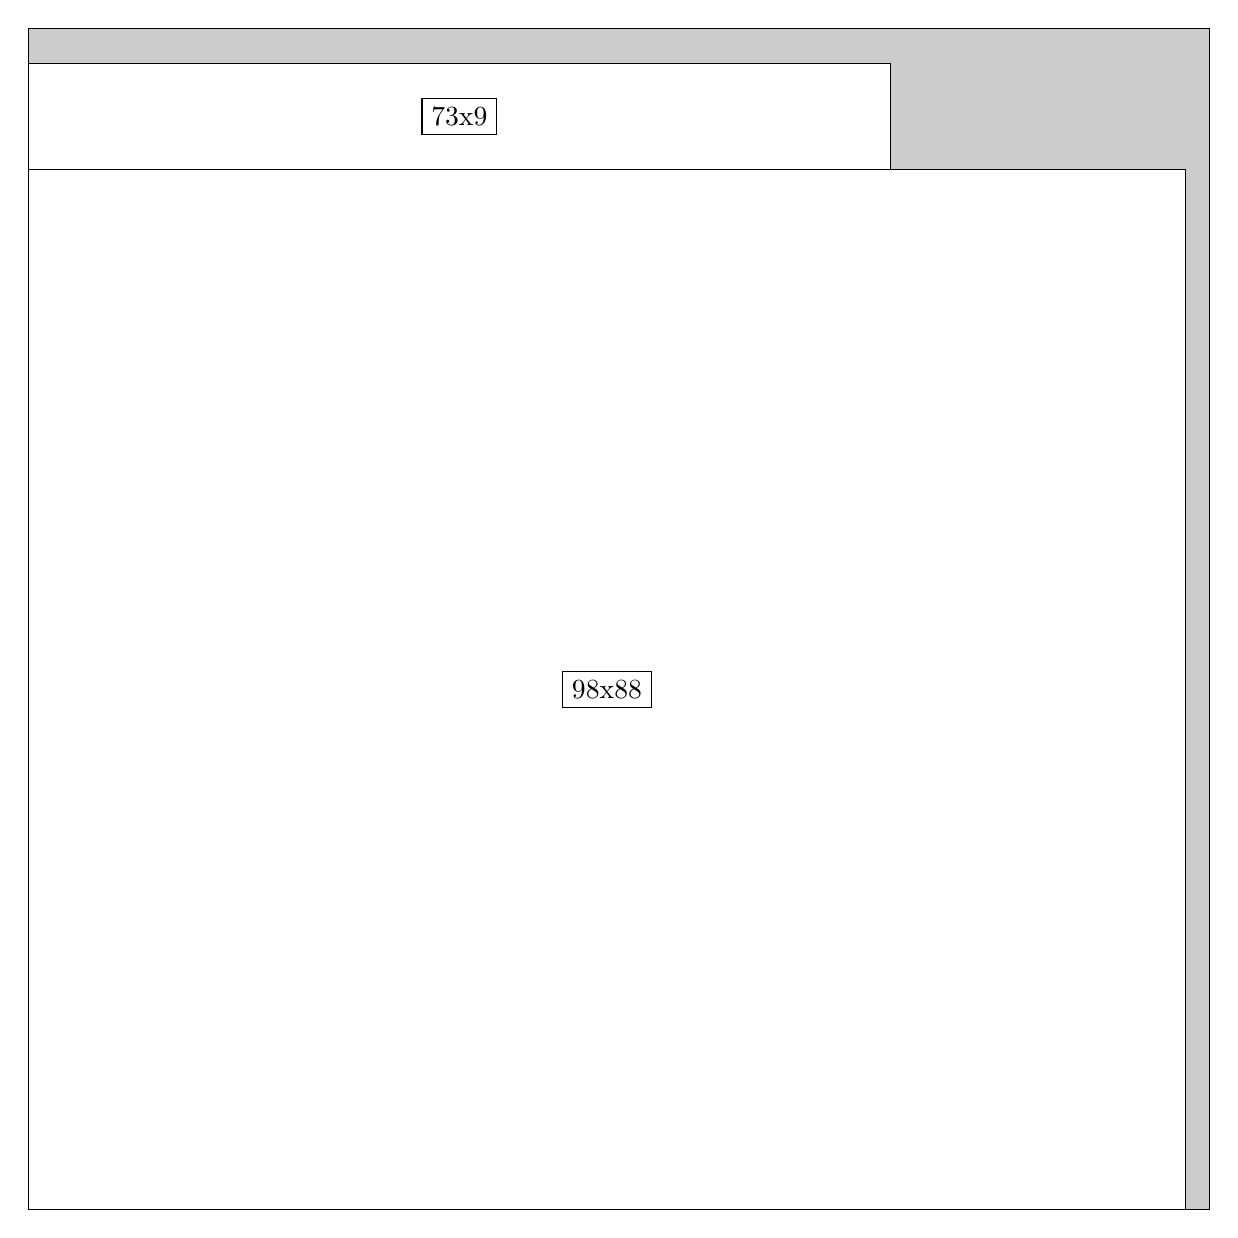
\begin{tikzpicture}[shorten >=1pt,scale=1.0,every node/.style={scale=1.0},->]
\tikzstyle{vertex}=[circle,fill=black!25,minimum size=14pt,inner sep=0pt]
\filldraw[fill=gray!40!white, draw=black] (0,0) rectangle (15.0,15.0);
\foreach \name/\x/\y/\w/\h in {98x88/0.0/0.0/14.7/13.2,73x9/0.0/13.2/10.95/1.3499999999999999}
\filldraw[fill=white!40!white, draw=black] (\x,\y) rectangle node[draw] (\name) {\name} ++(\w,\h);
\end{tikzpicture}


w =98 , h =88 , x =0 , y =0 , v =8624
\par
w =73 , h =9 , x =0 , y =88 , v =657
\par
\newpage


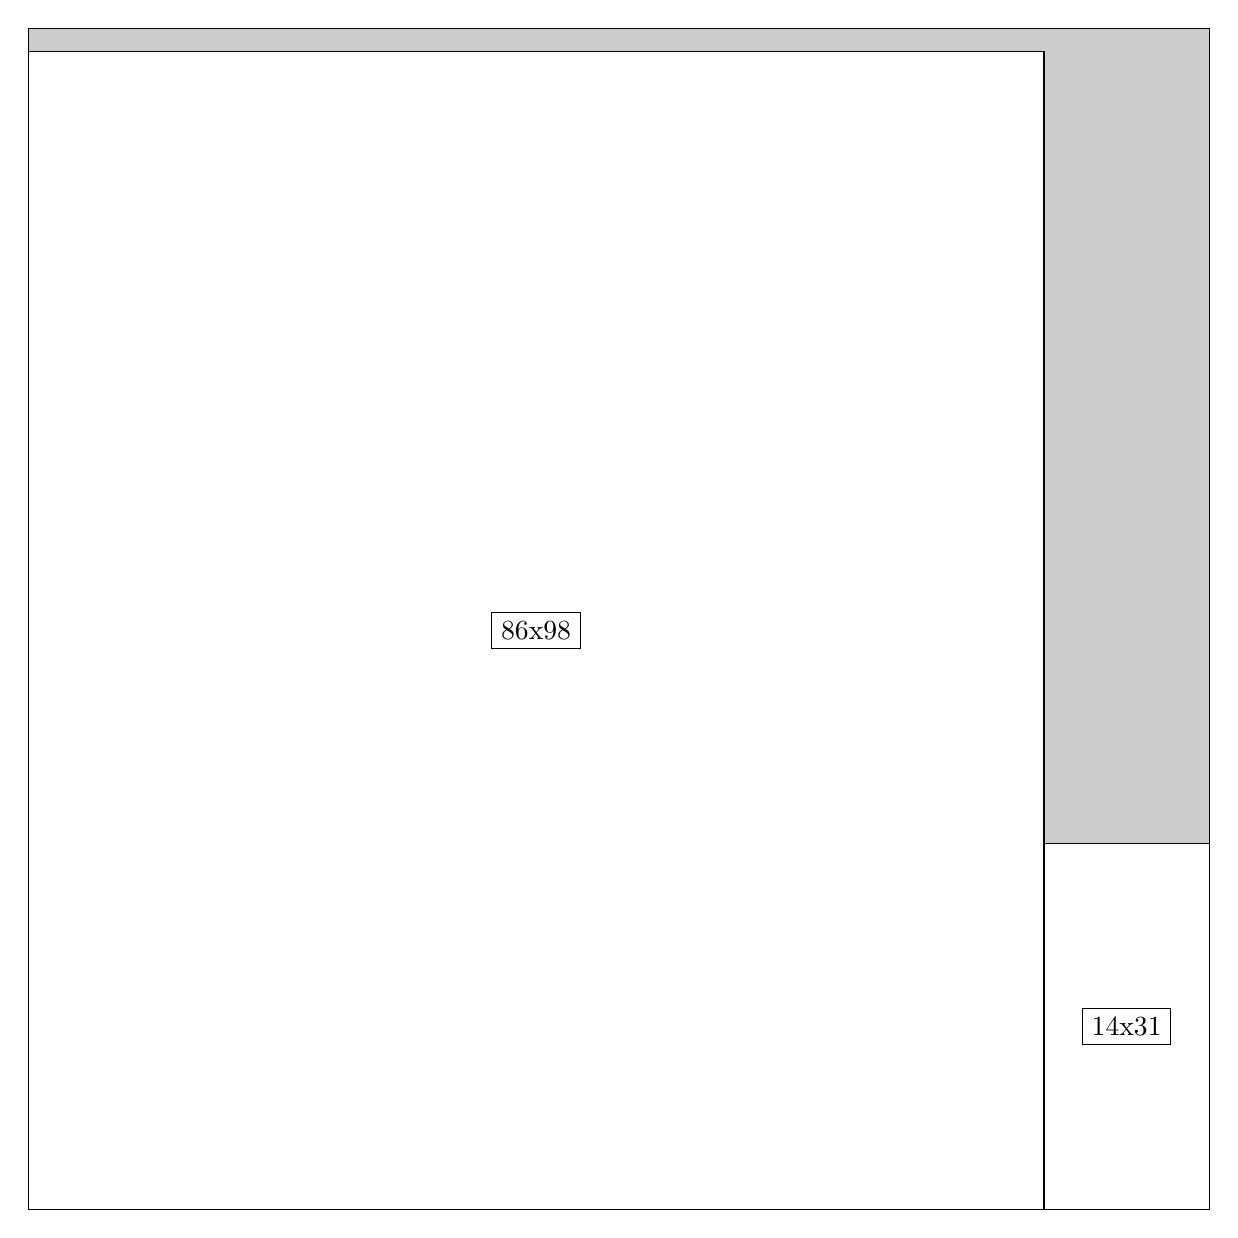
\begin{tikzpicture}[shorten >=1pt,scale=1.0,every node/.style={scale=1.0},->]
\tikzstyle{vertex}=[circle,fill=black!25,minimum size=14pt,inner sep=0pt]
\filldraw[fill=gray!40!white, draw=black] (0,0) rectangle (15.0,15.0);
\foreach \name/\x/\y/\w/\h in {86x98/0.0/0.0/12.9/14.7,14x31/12.9/0.0/2.1/4.6499999999999995}
\filldraw[fill=white!40!white, draw=black] (\x,\y) rectangle node[draw] (\name) {\name} ++(\w,\h);
\end{tikzpicture}


w =86 , h =98 , x =0 , y =0 , v =8428
\par
w =14 , h =31 , x =86 , y =0 , v =434
\par
\newpage


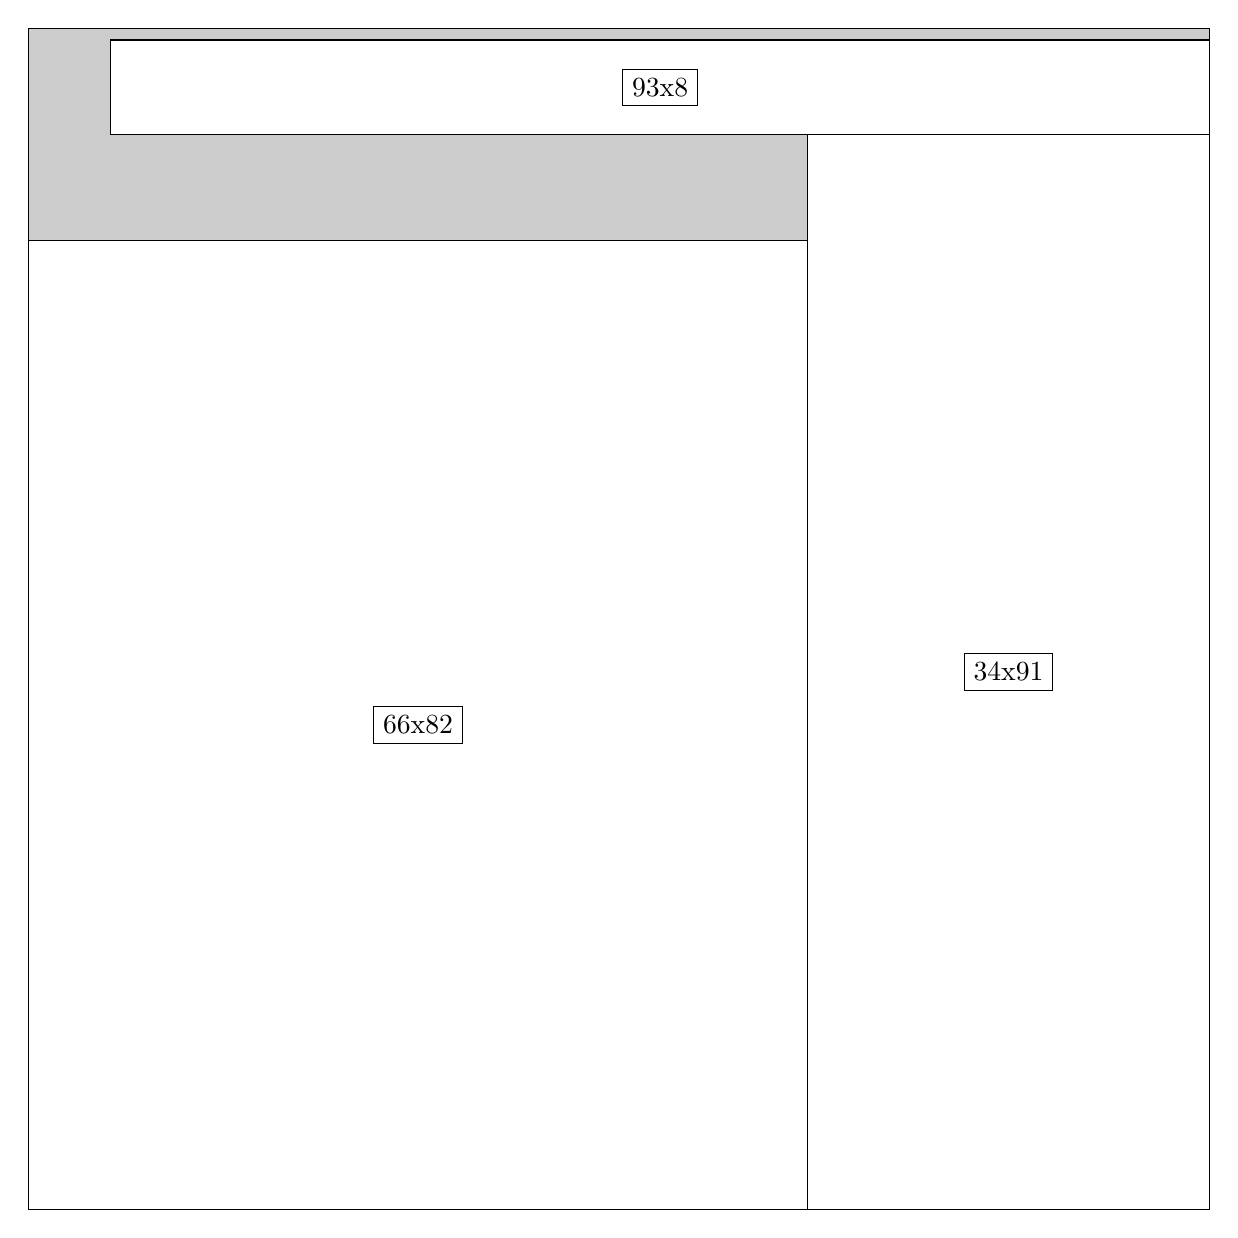
\begin{tikzpicture}[shorten >=1pt,scale=1.0,every node/.style={scale=1.0},->]
\tikzstyle{vertex}=[circle,fill=black!25,minimum size=14pt,inner sep=0pt]
\filldraw[fill=gray!40!white, draw=black] (0,0) rectangle (15.0,15.0);
\foreach \name/\x/\y/\w/\h in {66x82/0.0/0.0/9.9/12.299999999999999,34x91/9.9/0.0/5.1/13.65,93x8/1.05/13.65/13.95/1.2}
\filldraw[fill=white!40!white, draw=black] (\x,\y) rectangle node[draw] (\name) {\name} ++(\w,\h);
\end{tikzpicture}


w =66 , h =82 , x =0 , y =0 , v =5412
\par
w =34 , h =91 , x =66 , y =0 , v =3094
\par
w =93 , h =8 , x =7 , y =91 , v =744
\par
\newpage


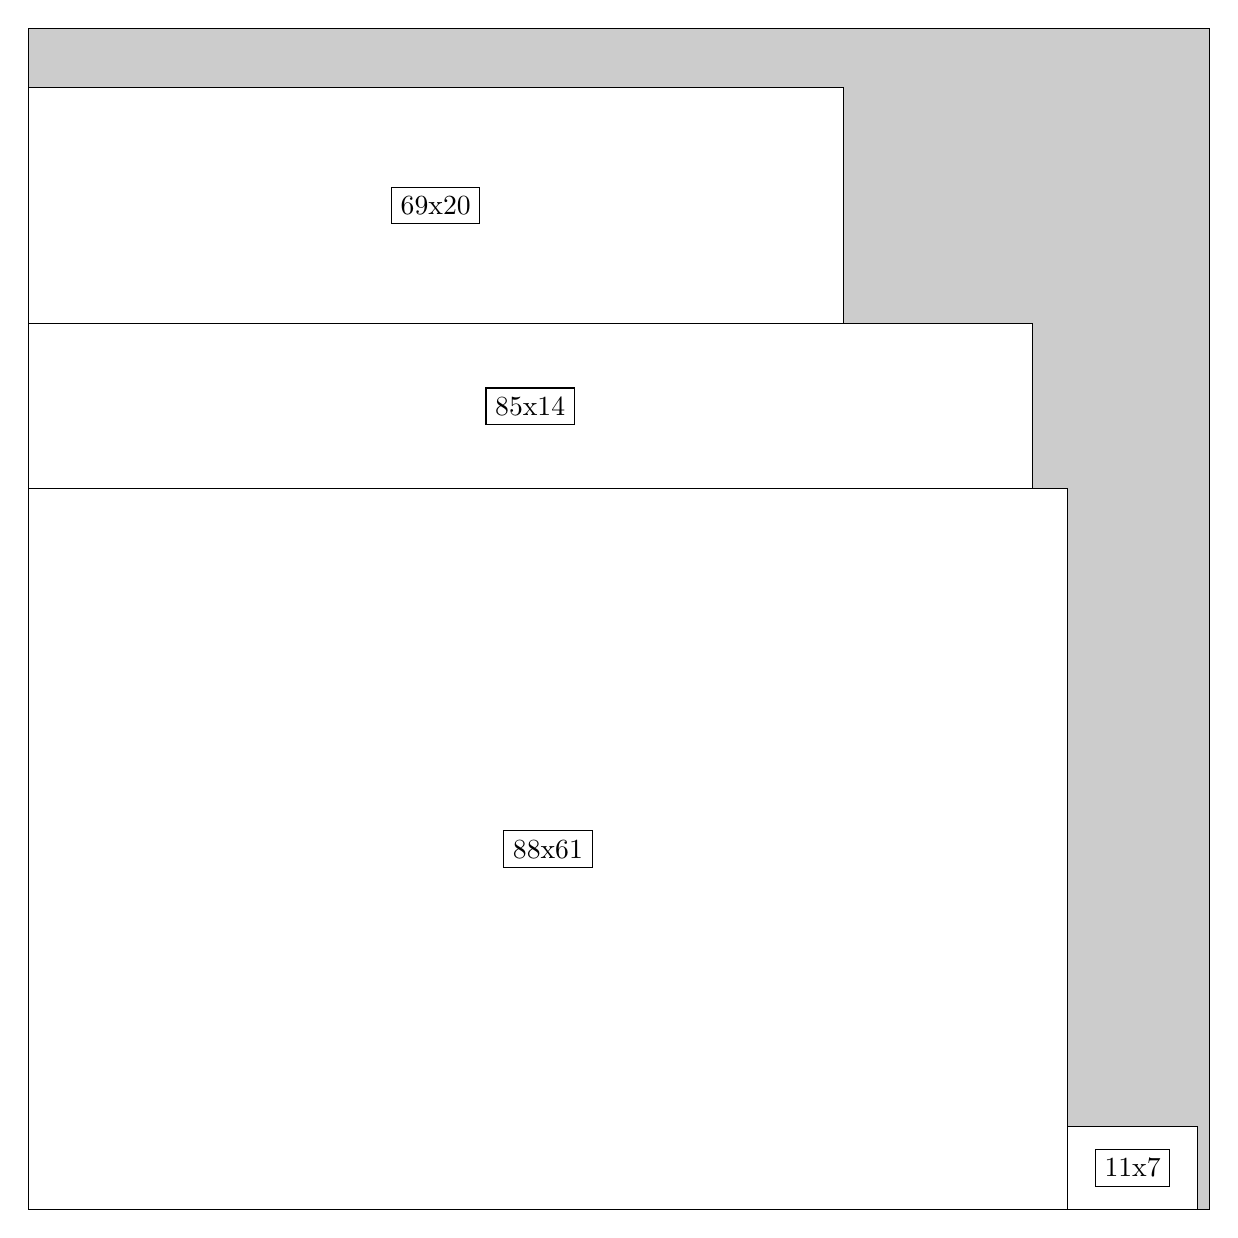
\begin{tikzpicture}[shorten >=1pt,scale=1.0,every node/.style={scale=1.0},->]
\tikzstyle{vertex}=[circle,fill=black!25,minimum size=14pt,inner sep=0pt]
\filldraw[fill=gray!40!white, draw=black] (0,0) rectangle (15.0,15.0);
\foreach \name/\x/\y/\w/\h in {88x61/0.0/0.0/13.2/9.15,69x20/0.0/11.25/10.35/3.0,85x14/0.0/9.15/12.75/2.1,11x7/13.2/0.0/1.65/1.05}
\filldraw[fill=white!40!white, draw=black] (\x,\y) rectangle node[draw] (\name) {\name} ++(\w,\h);
\end{tikzpicture}


w =88 , h =61 , x =0 , y =0 , v =5368
\par
w =69 , h =20 , x =0 , y =75 , v =1380
\par
w =85 , h =14 , x =0 , y =61 , v =1190
\par
w =11 , h =7 , x =88 , y =0 , v =77
\par
\newpage


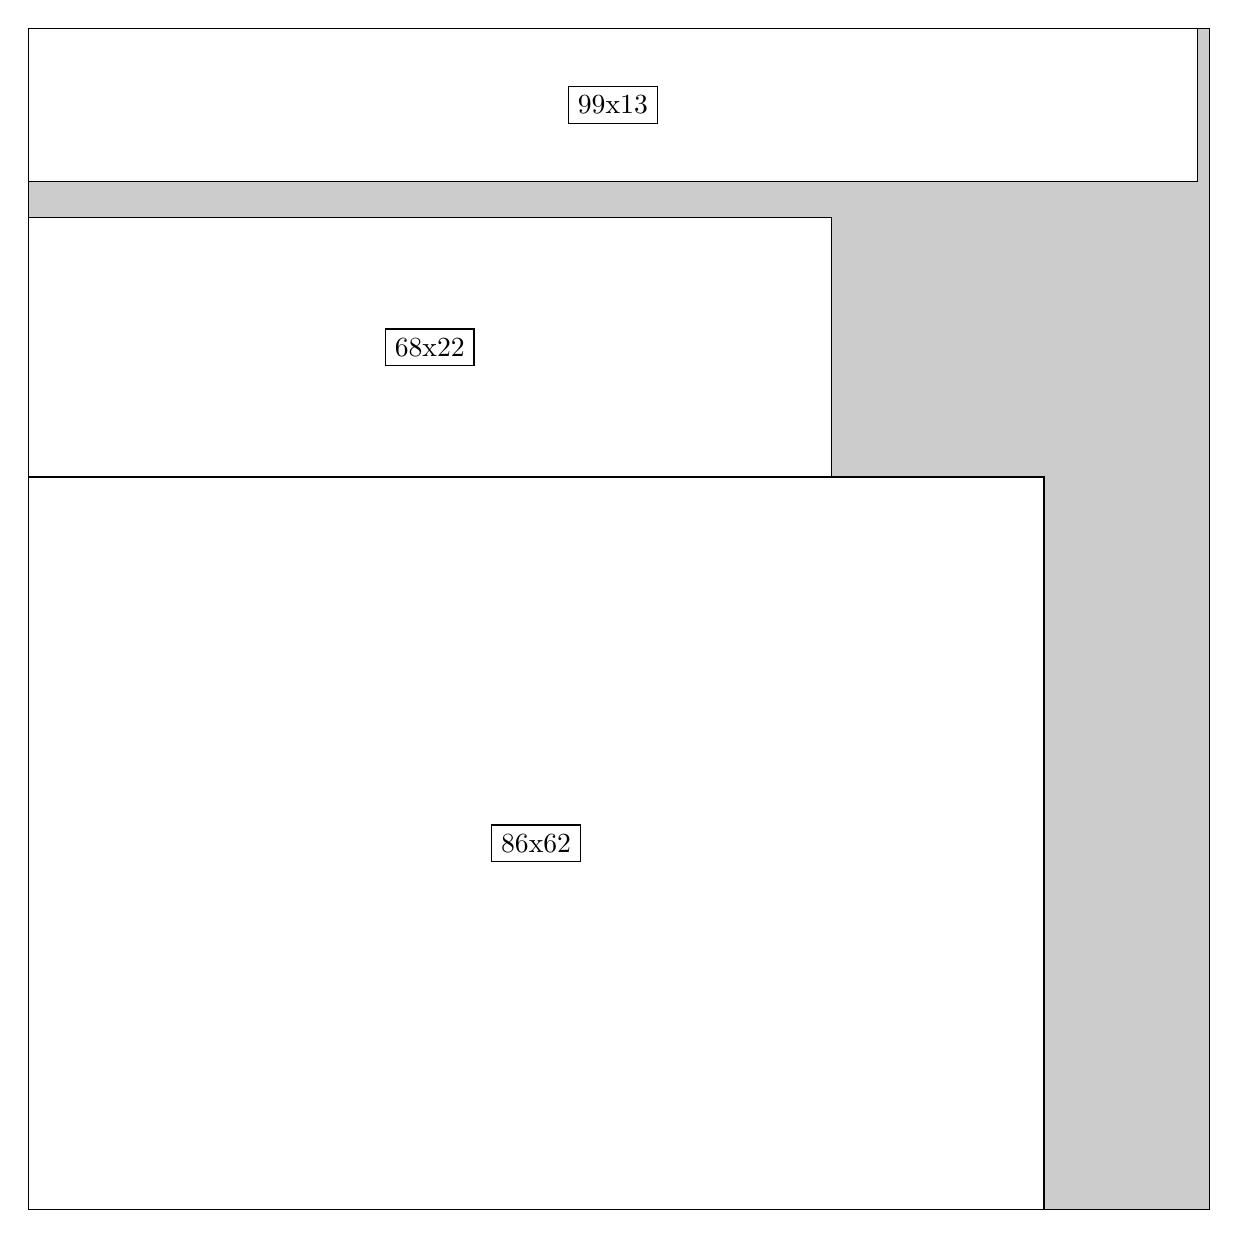
\begin{tikzpicture}[shorten >=1pt,scale=1.0,every node/.style={scale=1.0},->]
\tikzstyle{vertex}=[circle,fill=black!25,minimum size=14pt,inner sep=0pt]
\filldraw[fill=gray!40!white, draw=black] (0,0) rectangle (15.0,15.0);
\foreach \name/\x/\y/\w/\h in {86x62/0.0/0.0/12.9/9.299999999999999,68x22/0.0/9.299999999999999/10.2/3.3,99x13/0.0/13.049999999999999/14.85/1.95}
\filldraw[fill=white!40!white, draw=black] (\x,\y) rectangle node[draw] (\name) {\name} ++(\w,\h);
\end{tikzpicture}


w =86 , h =62 , x =0 , y =0 , v =5332
\par
w =68 , h =22 , x =0 , y =62 , v =1496
\par
w =99 , h =13 , x =0 , y =87 , v =1287
\par
\newpage


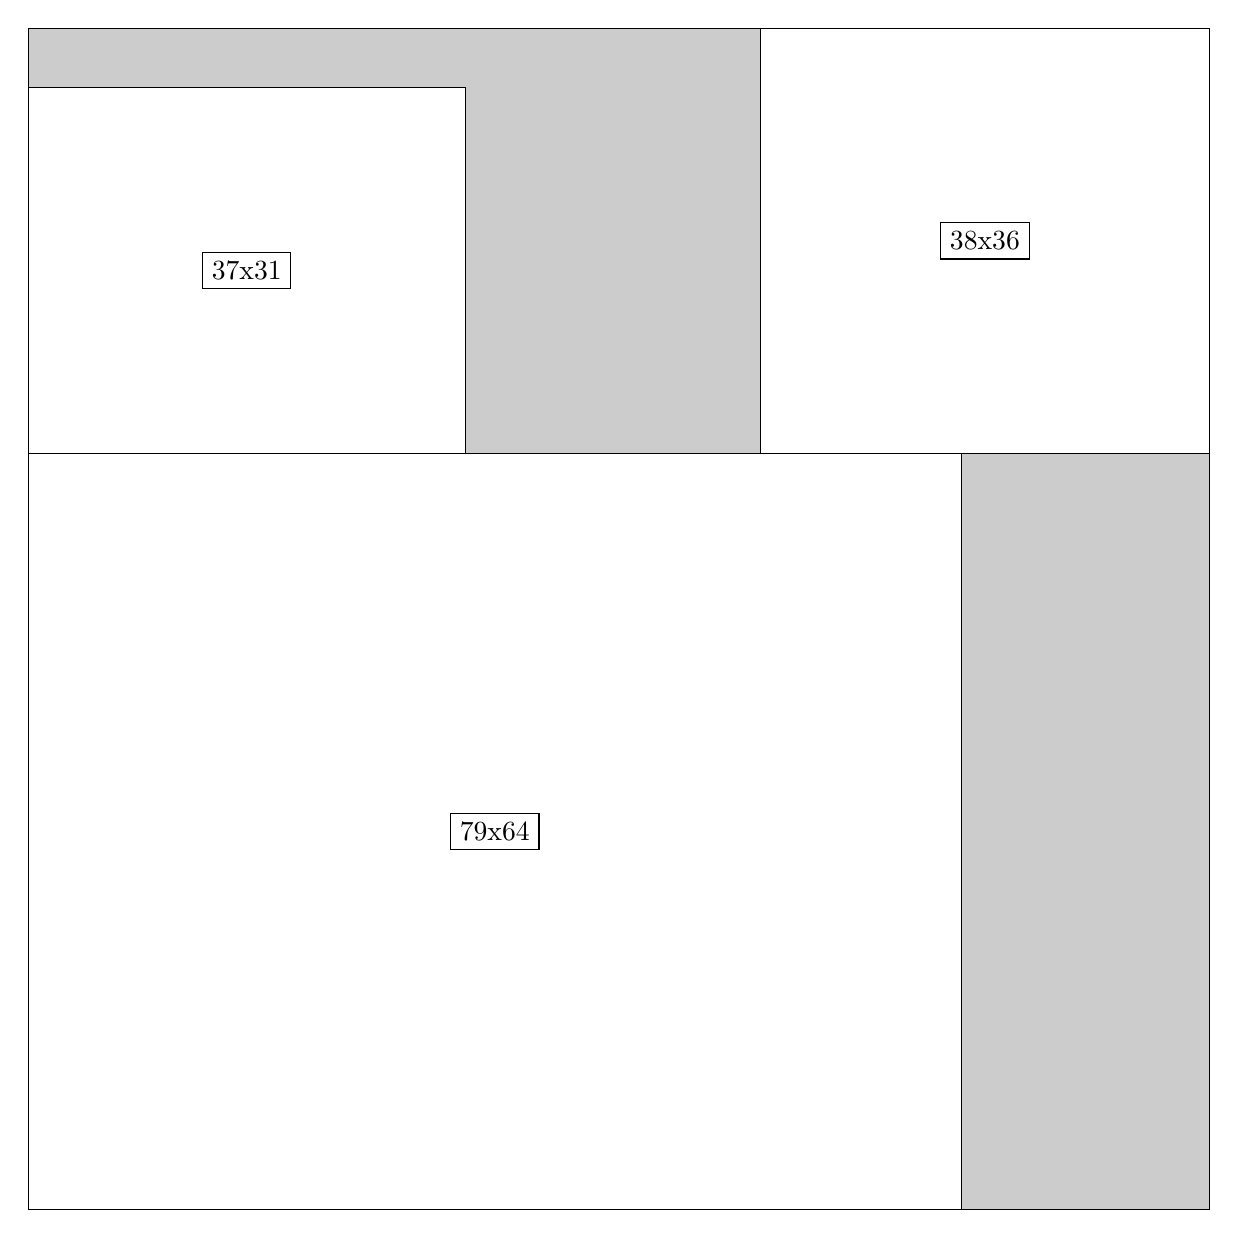
\begin{tikzpicture}[shorten >=1pt,scale=1.0,every node/.style={scale=1.0},->]
\tikzstyle{vertex}=[circle,fill=black!25,minimum size=14pt,inner sep=0pt]
\filldraw[fill=gray!40!white, draw=black] (0,0) rectangle (15.0,15.0);
\foreach \name/\x/\y/\w/\h in {79x64/0.0/0.0/11.85/9.6,38x36/9.299999999999999/9.6/5.7/5.3999999999999995,37x31/0.0/9.6/5.55/4.6499999999999995}
\filldraw[fill=white!40!white, draw=black] (\x,\y) rectangle node[draw] (\name) {\name} ++(\w,\h);
\end{tikzpicture}


w =79 , h =64 , x =0 , y =0 , v =5056
\par
w =38 , h =36 , x =62 , y =64 , v =1368
\par
w =37 , h =31 , x =0 , y =64 , v =1147
\par
\newpage


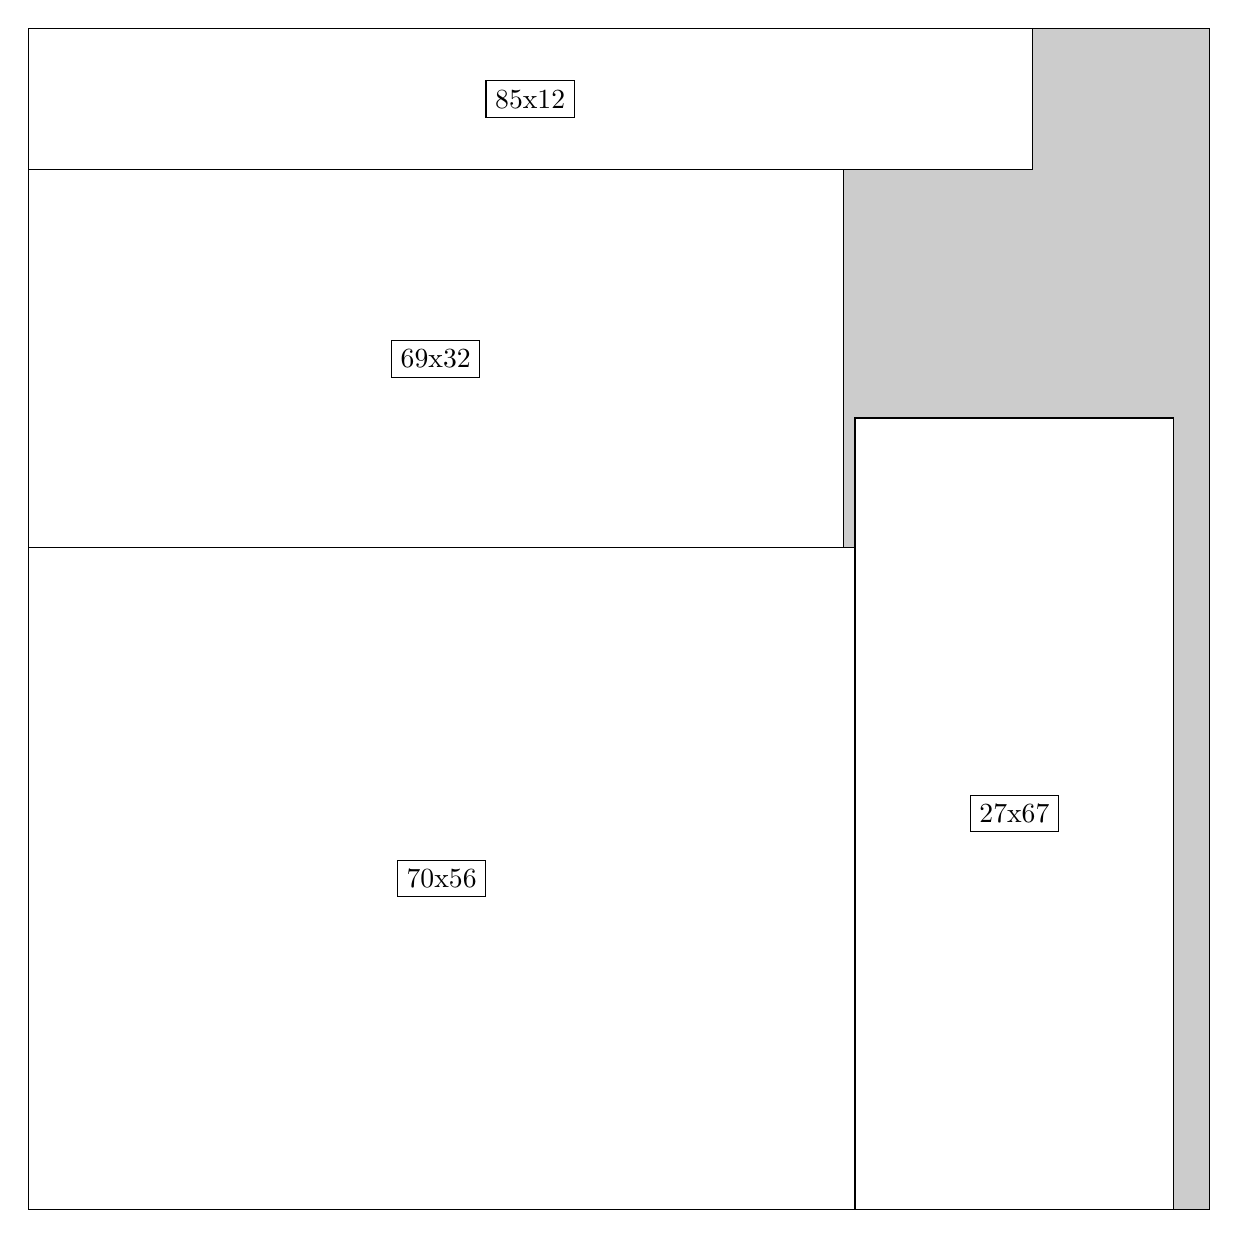
\begin{tikzpicture}[shorten >=1pt,scale=1.0,every node/.style={scale=1.0},->]
\tikzstyle{vertex}=[circle,fill=black!25,minimum size=14pt,inner sep=0pt]
\filldraw[fill=gray!40!white, draw=black] (0,0) rectangle (15.0,15.0);
\foreach \name/\x/\y/\w/\h in {70x56/0.0/0.0/10.5/8.4,69x32/0.0/8.4/10.35/4.8,27x67/10.5/0.0/4.05/10.049999999999999,85x12/0.0/13.2/12.75/1.7999999999999998}
\filldraw[fill=white!40!white, draw=black] (\x,\y) rectangle node[draw] (\name) {\name} ++(\w,\h);
\end{tikzpicture}


w =70 , h =56 , x =0 , y =0 , v =3920
\par
w =69 , h =32 , x =0 , y =56 , v =2208
\par
w =27 , h =67 , x =70 , y =0 , v =1809
\par
w =85 , h =12 , x =0 , y =88 , v =1020
\par
\newpage


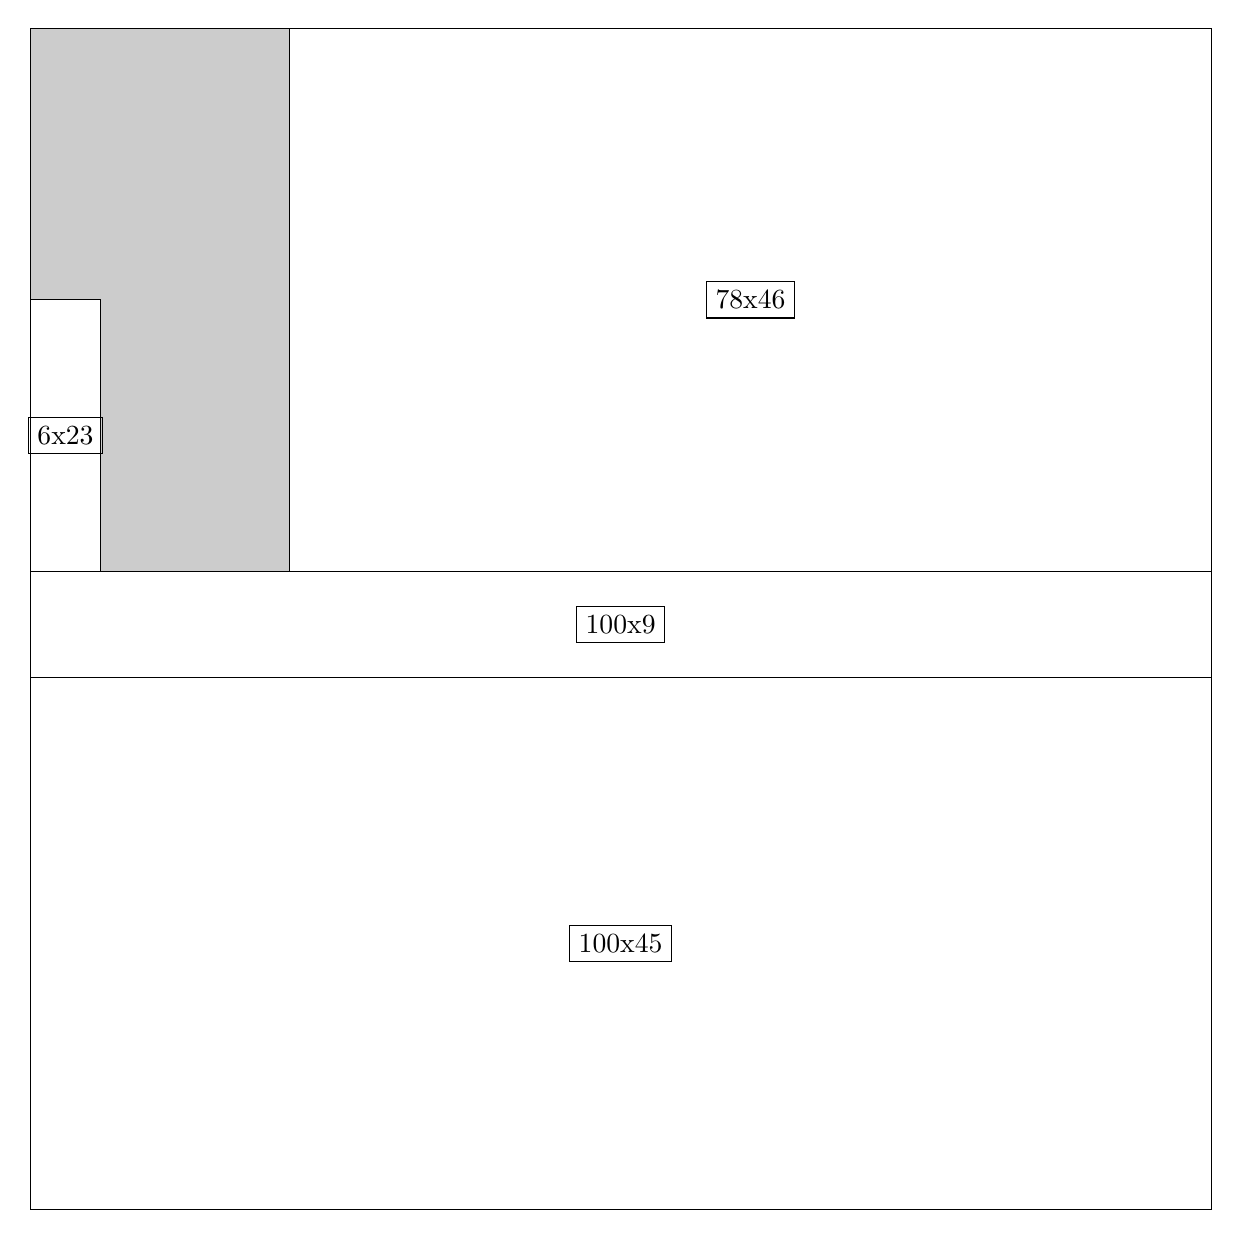
\begin{tikzpicture}[shorten >=1pt,scale=1.0,every node/.style={scale=1.0},->]
\tikzstyle{vertex}=[circle,fill=black!25,minimum size=14pt,inner sep=0pt]
\filldraw[fill=gray!40!white, draw=black] (0,0) rectangle (15.0,15.0);
\foreach \name/\x/\y/\w/\h in {100x45/0.0/0.0/15.0/6.75,78x46/3.3/8.1/11.7/6.8999999999999995,100x9/0.0/6.75/15.0/1.3499999999999999,6x23/0.0/8.1/0.8999999999999999/3.4499999999999997}
\filldraw[fill=white!40!white, draw=black] (\x,\y) rectangle node[draw] (\name) {\name} ++(\w,\h);
\end{tikzpicture}


w =100 , h =45 , x =0 , y =0 , v =4500
\par
w =78 , h =46 , x =22 , y =54 , v =3588
\par
w =100 , h =9 , x =0 , y =45 , v =900
\par
w =6 , h =23 , x =0 , y =54 , v =138
\par
\newpage


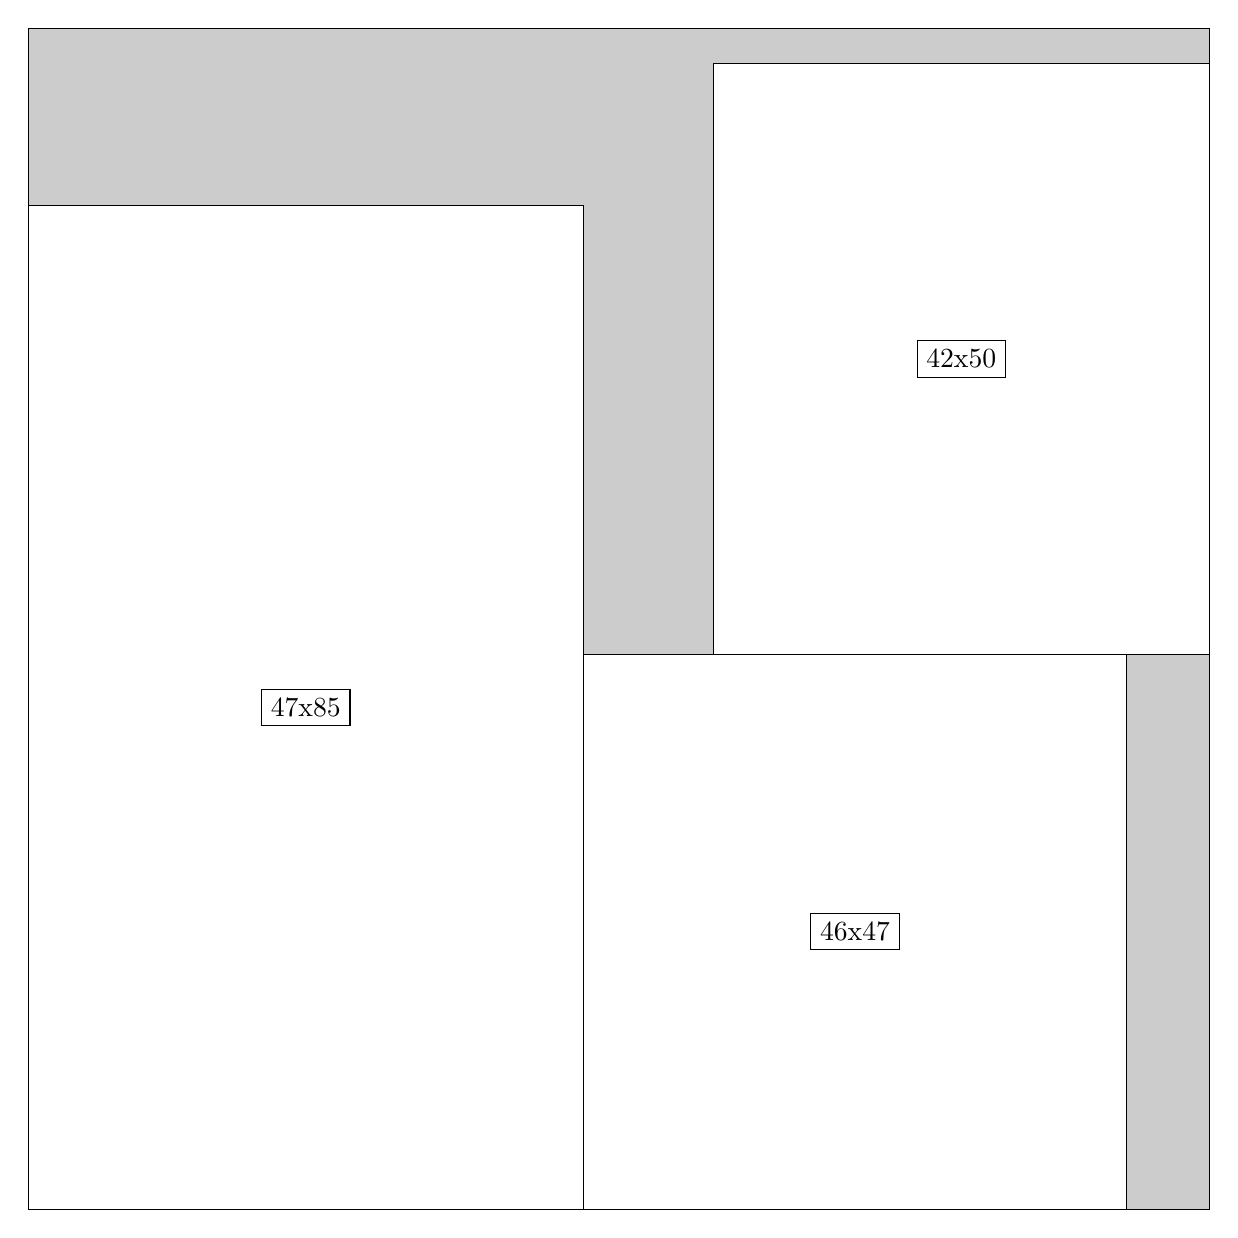
\begin{tikzpicture}[shorten >=1pt,scale=1.0,every node/.style={scale=1.0},->]
\tikzstyle{vertex}=[circle,fill=black!25,minimum size=14pt,inner sep=0pt]
\filldraw[fill=gray!40!white, draw=black] (0,0) rectangle (15.0,15.0);
\foreach \name/\x/\y/\w/\h in {47x85/0.0/0.0/7.05/12.75,46x47/7.05/0.0/6.8999999999999995/7.05,42x50/8.7/7.05/6.3/7.5}
\filldraw[fill=white!40!white, draw=black] (\x,\y) rectangle node[draw] (\name) {\name} ++(\w,\h);
\end{tikzpicture}


w =47 , h =85 , x =0 , y =0 , v =3995
\par
w =46 , h =47 , x =47 , y =0 , v =2162
\par
w =42 , h =50 , x =58 , y =47 , v =2100
\par
\newpage


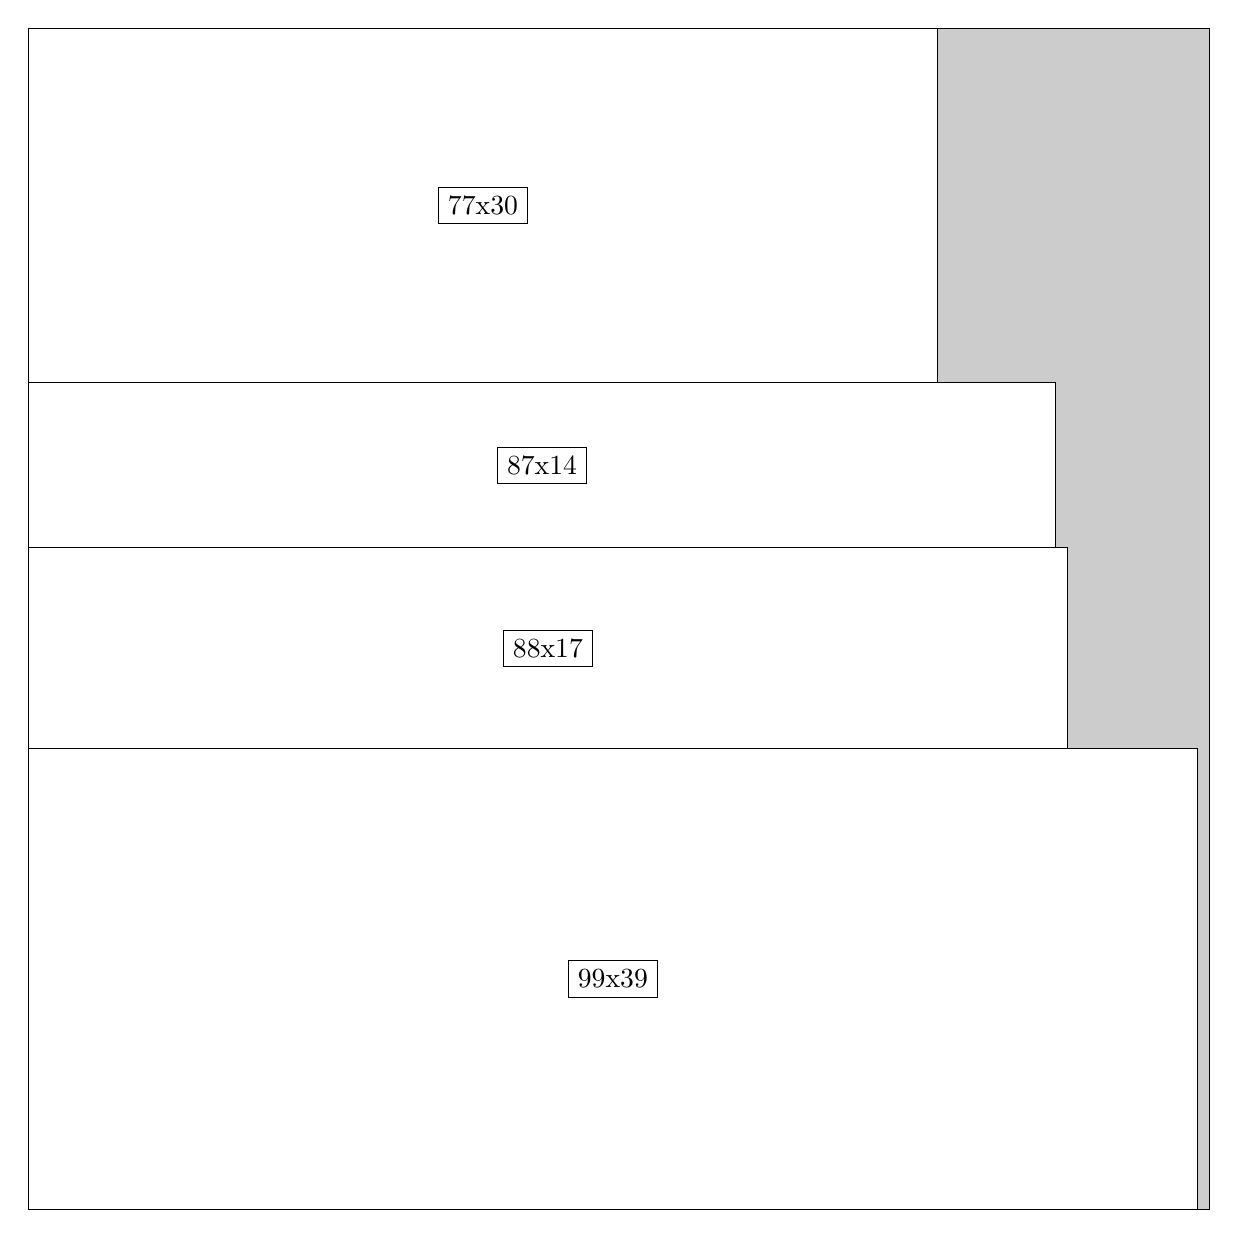
\begin{tikzpicture}[shorten >=1pt,scale=1.0,every node/.style={scale=1.0},->]
\tikzstyle{vertex}=[circle,fill=black!25,minimum size=14pt,inner sep=0pt]
\filldraw[fill=gray!40!white, draw=black] (0,0) rectangle (15.0,15.0);
\foreach \name/\x/\y/\w/\h in {99x39/0.0/0.0/14.85/5.85,77x30/0.0/10.5/11.549999999999999/4.5,88x17/0.0/5.85/13.2/2.55,87x14/0.0/8.4/13.049999999999999/2.1}
\filldraw[fill=white!40!white, draw=black] (\x,\y) rectangle node[draw] (\name) {\name} ++(\w,\h);
\end{tikzpicture}


w =99 , h =39 , x =0 , y =0 , v =3861
\par
w =77 , h =30 , x =0 , y =70 , v =2310
\par
w =88 , h =17 , x =0 , y =39 , v =1496
\par
w =87 , h =14 , x =0 , y =56 , v =1218
\par
\newpage


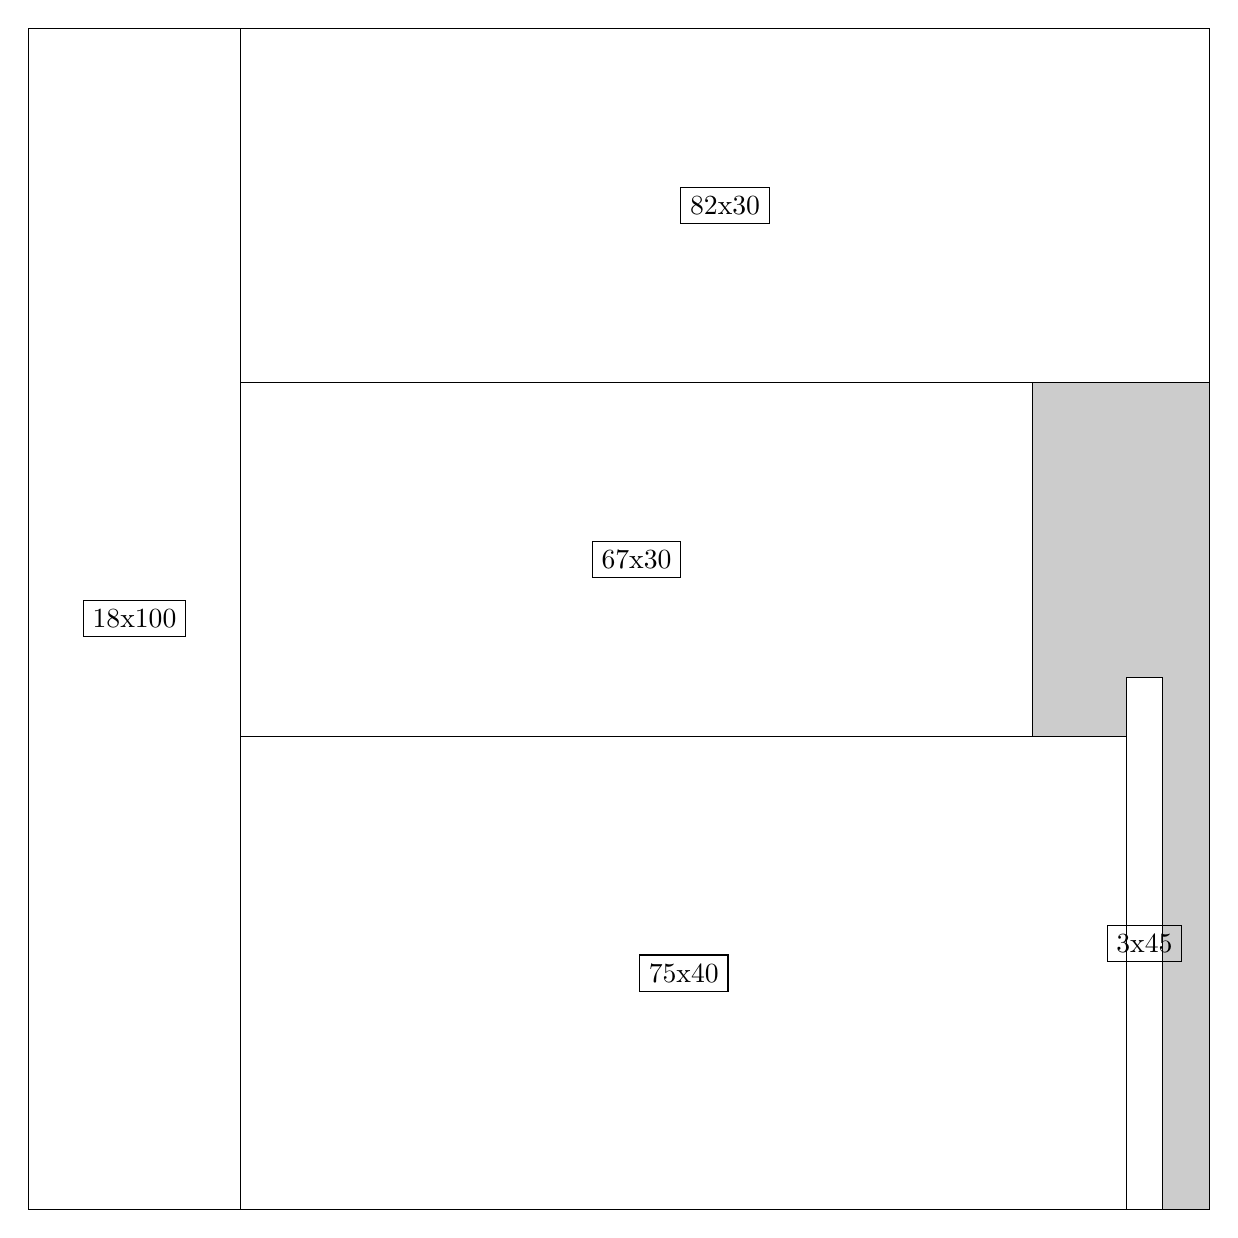
\begin{tikzpicture}[shorten >=1pt,scale=1.0,every node/.style={scale=1.0},->]
\tikzstyle{vertex}=[circle,fill=black!25,minimum size=14pt,inner sep=0pt]
\filldraw[fill=gray!40!white, draw=black] (0,0) rectangle (15.0,15.0);
\foreach \name/\x/\y/\w/\h in {75x40/2.6999999999999997/0.0/11.25/6.0,82x30/2.6999999999999997/10.5/12.299999999999999/4.5,67x30/2.6999999999999997/6.0/10.049999999999999/4.5,18x100/0.0/0.0/2.6999999999999997/15.0,3x45/13.95/0.0/0.44999999999999996/6.75}
\filldraw[fill=white!40!white, draw=black] (\x,\y) rectangle node[draw] (\name) {\name} ++(\w,\h);
\end{tikzpicture}


w =75 , h =40 , x =18 , y =0 , v =3000
\par
w =82 , h =30 , x =18 , y =70 , v =2460
\par
w =67 , h =30 , x =18 , y =40 , v =2010
\par
w =18 , h =100 , x =0 , y =0 , v =1800
\par
w =3 , h =45 , x =93 , y =0 , v =135
\par
\newpage


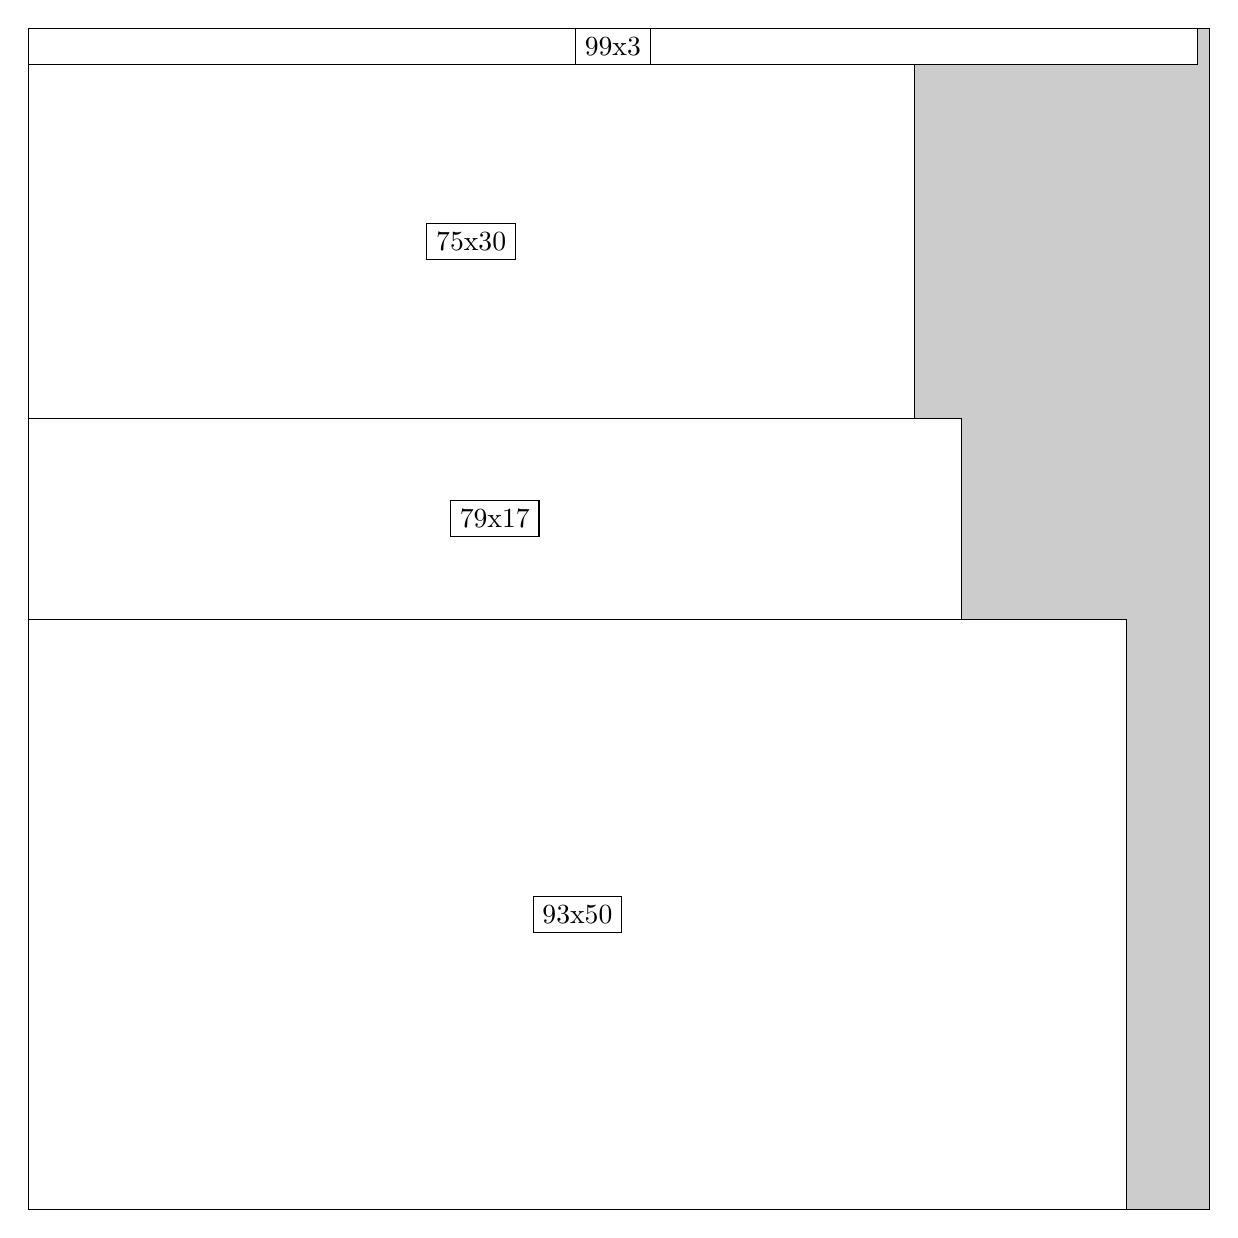
\begin{tikzpicture}[shorten >=1pt,scale=1.0,every node/.style={scale=1.0},->]
\tikzstyle{vertex}=[circle,fill=black!25,minimum size=14pt,inner sep=0pt]
\filldraw[fill=gray!40!white, draw=black] (0,0) rectangle (15.0,15.0);
\foreach \name/\x/\y/\w/\h in {93x50/0.0/0.0/13.95/7.5,99x3/0.0/14.549999999999999/14.85/0.44999999999999996,75x30/0.0/10.049999999999999/11.25/4.5,79x17/0.0/7.5/11.85/2.55}
\filldraw[fill=white!40!white, draw=black] (\x,\y) rectangle node[draw] (\name) {\name} ++(\w,\h);
\end{tikzpicture}


w =93 , h =50 , x =0 , y =0 , v =4650
\par
w =99 , h =3 , x =0 , y =97 , v =297
\par
w =75 , h =30 , x =0 , y =67 , v =2250
\par
w =79 , h =17 , x =0 , y =50 , v =1343
\par
\newpage


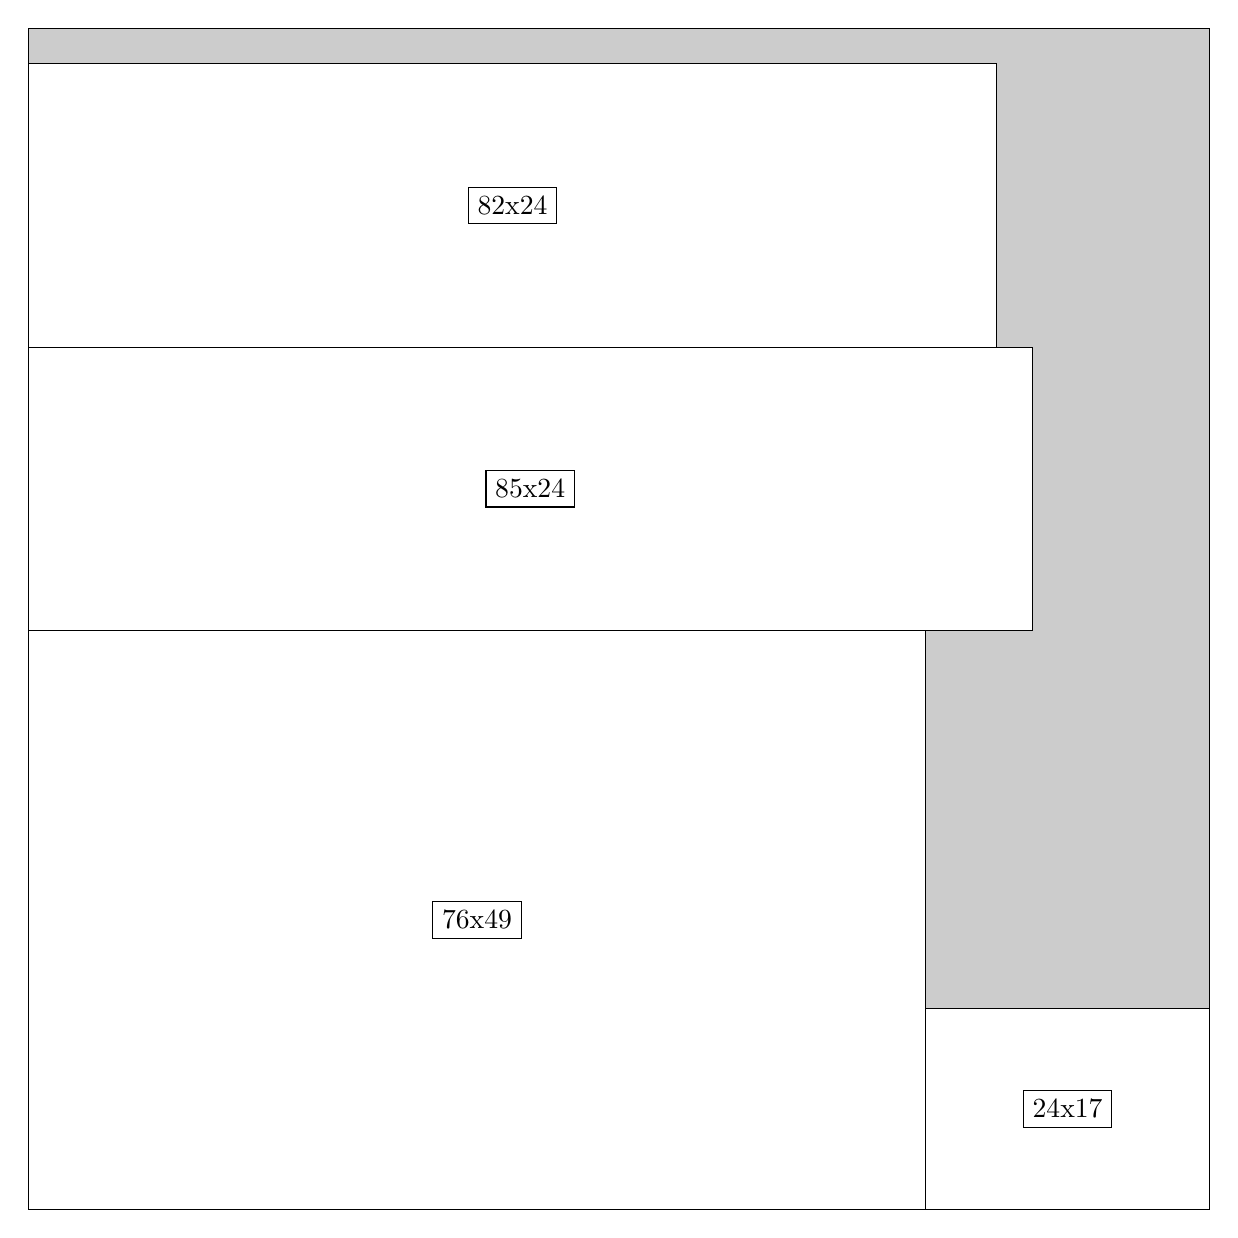
\begin{tikzpicture}[shorten >=1pt,scale=1.0,every node/.style={scale=1.0},->]
\tikzstyle{vertex}=[circle,fill=black!25,minimum size=14pt,inner sep=0pt]
\filldraw[fill=gray!40!white, draw=black] (0,0) rectangle (15.0,15.0);
\foreach \name/\x/\y/\w/\h in {76x49/0.0/0.0/11.4/7.35,85x24/0.0/7.35/12.75/3.5999999999999996,82x24/0.0/10.95/12.299999999999999/3.5999999999999996,24x17/11.4/0.0/3.5999999999999996/2.55}
\filldraw[fill=white!40!white, draw=black] (\x,\y) rectangle node[draw] (\name) {\name} ++(\w,\h);
\end{tikzpicture}


w =76 , h =49 , x =0 , y =0 , v =3724
\par
w =85 , h =24 , x =0 , y =49 , v =2040
\par
w =82 , h =24 , x =0 , y =73 , v =1968
\par
w =24 , h =17 , x =76 , y =0 , v =408
\par
\newpage


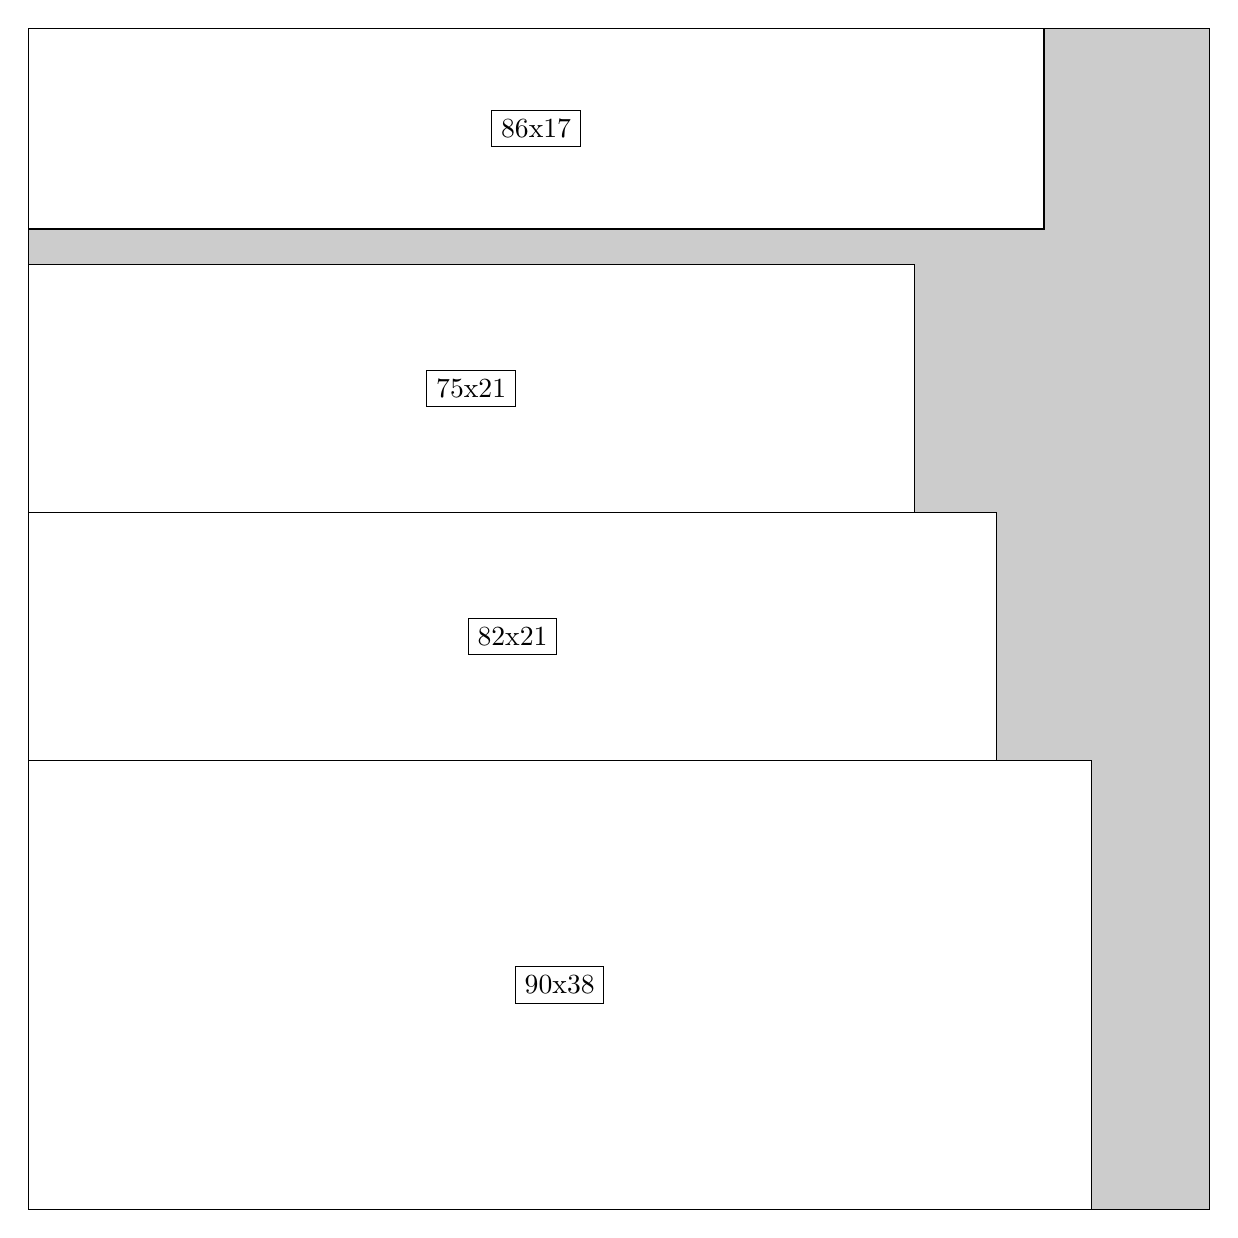
\begin{tikzpicture}[shorten >=1pt,scale=1.0,every node/.style={scale=1.0},->]
\tikzstyle{vertex}=[circle,fill=black!25,minimum size=14pt,inner sep=0pt]
\filldraw[fill=gray!40!white, draw=black] (0,0) rectangle (15.0,15.0);
\foreach \name/\x/\y/\w/\h in {90x38/0.0/0.0/13.5/5.7,86x17/0.0/12.45/12.9/2.55,82x21/0.0/5.7/12.299999999999999/3.15,75x21/0.0/8.85/11.25/3.15}
\filldraw[fill=white!40!white, draw=black] (\x,\y) rectangle node[draw] (\name) {\name} ++(\w,\h);
\end{tikzpicture}


w =90 , h =38 , x =0 , y =0 , v =3420
\par
w =86 , h =17 , x =0 , y =83 , v =1462
\par
w =82 , h =21 , x =0 , y =38 , v =1722
\par
w =75 , h =21 , x =0 , y =59 , v =1575
\par
\newpage


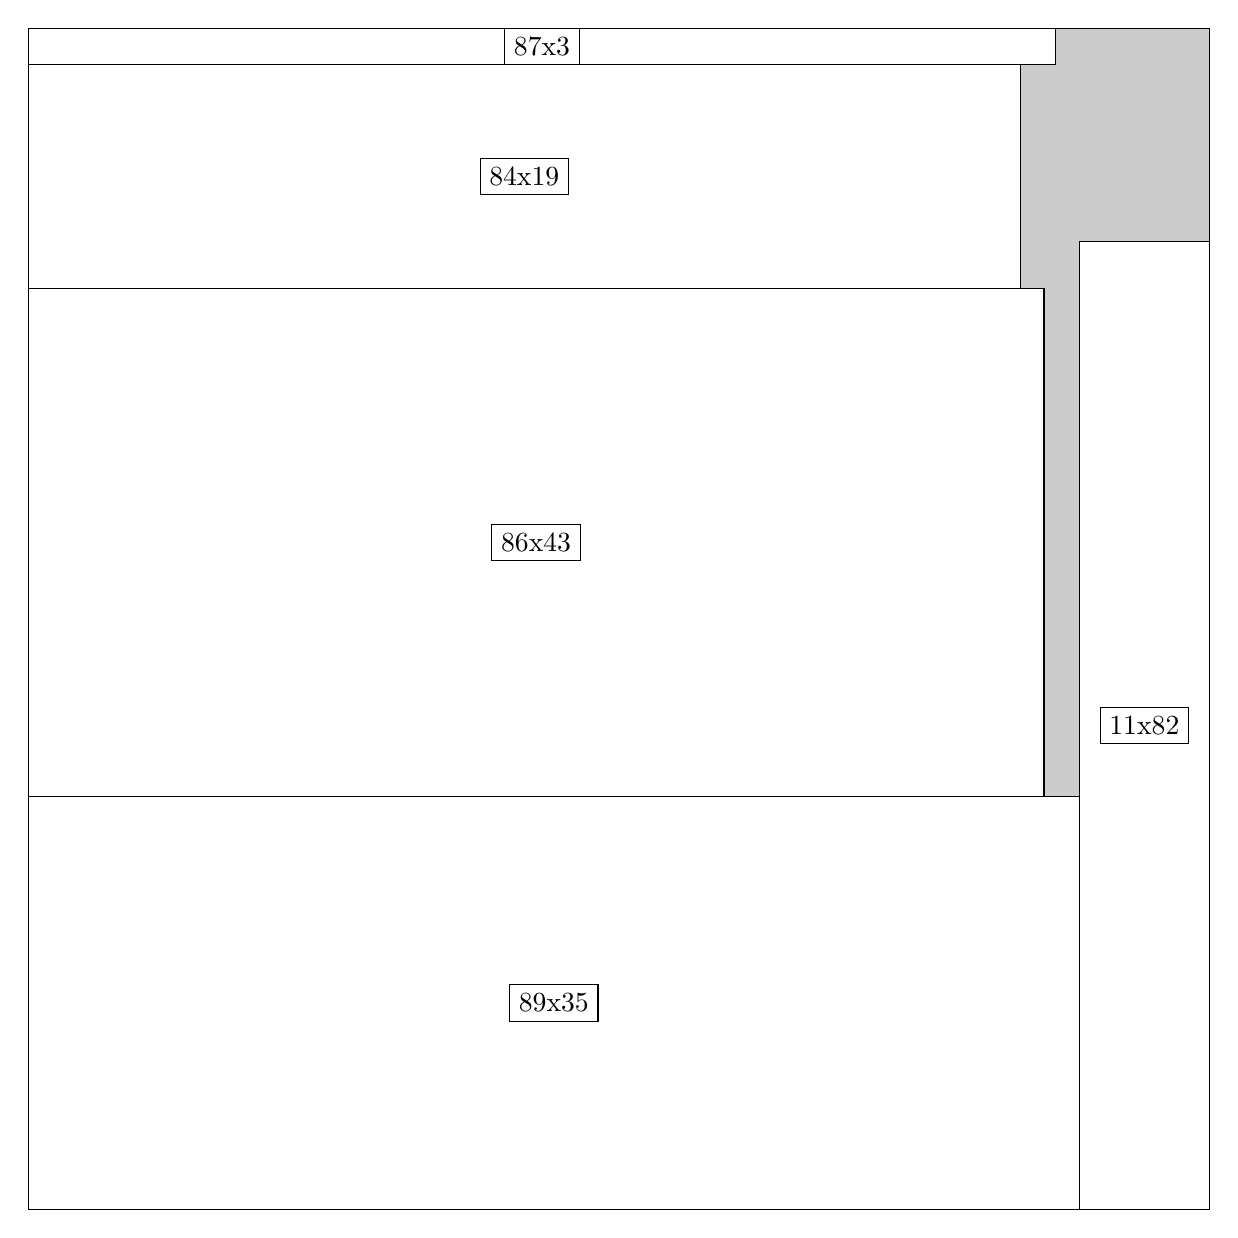
\begin{tikzpicture}[shorten >=1pt,scale=1.0,every node/.style={scale=1.0},->]
\tikzstyle{vertex}=[circle,fill=black!25,minimum size=14pt,inner sep=0pt]
\filldraw[fill=gray!40!white, draw=black] (0,0) rectangle (15.0,15.0);
\foreach \name/\x/\y/\w/\h in {89x35/0.0/0.0/13.35/5.25,86x43/0.0/5.25/12.9/6.45,84x19/0.0/11.7/12.6/2.85,11x82/13.35/0.0/1.65/12.299999999999999,87x3/0.0/14.549999999999999/13.049999999999999/0.44999999999999996}
\filldraw[fill=white!40!white, draw=black] (\x,\y) rectangle node[draw] (\name) {\name} ++(\w,\h);
\end{tikzpicture}


w =89 , h =35 , x =0 , y =0 , v =3115
\par
w =86 , h =43 , x =0 , y =35 , v =3698
\par
w =84 , h =19 , x =0 , y =78 , v =1596
\par
w =11 , h =82 , x =89 , y =0 , v =902
\par
w =87 , h =3 , x =0 , y =97 , v =261
\par
\newpage


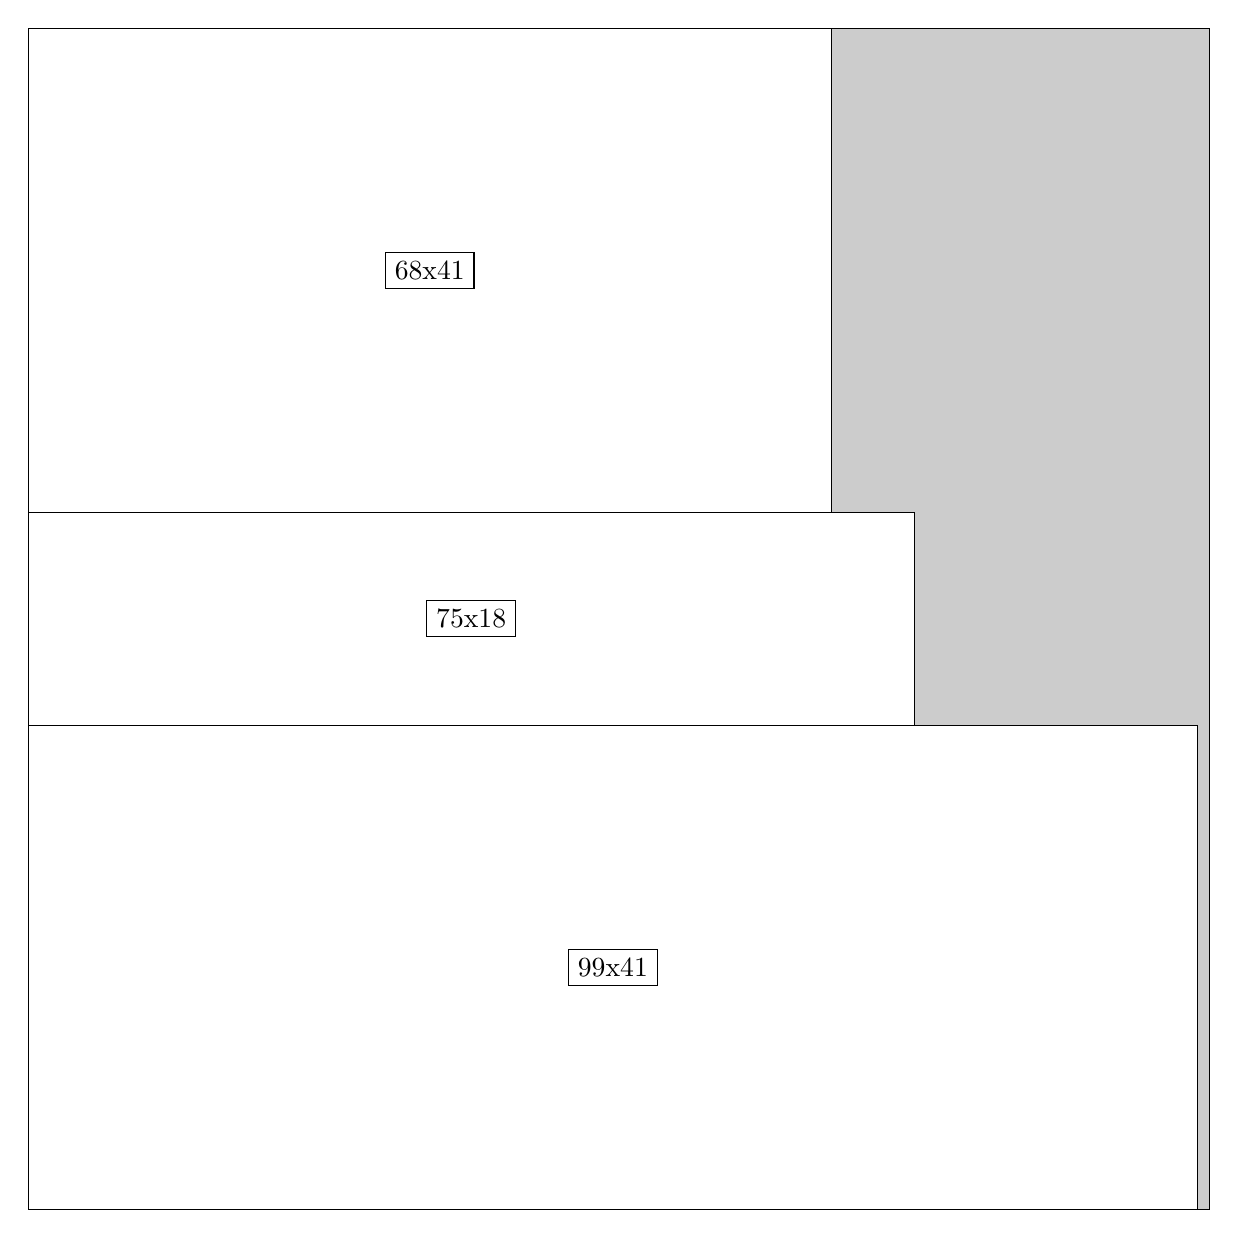
\begin{tikzpicture}[shorten >=1pt,scale=1.0,every node/.style={scale=1.0},->]
\tikzstyle{vertex}=[circle,fill=black!25,minimum size=14pt,inner sep=0pt]
\filldraw[fill=gray!40!white, draw=black] (0,0) rectangle (15.0,15.0);
\foreach \name/\x/\y/\w/\h in {99x41/0.0/0.0/14.85/6.1499999999999995,68x41/0.0/8.85/10.2/6.1499999999999995,75x18/0.0/6.1499999999999995/11.25/2.6999999999999997}
\filldraw[fill=white!40!white, draw=black] (\x,\y) rectangle node[draw] (\name) {\name} ++(\w,\h);
\end{tikzpicture}


w =99 , h =41 , x =0 , y =0 , v =4059
\par
w =68 , h =41 , x =0 , y =59 , v =2788
\par
w =75 , h =18 , x =0 , y =41 , v =1350
\par
\newpage


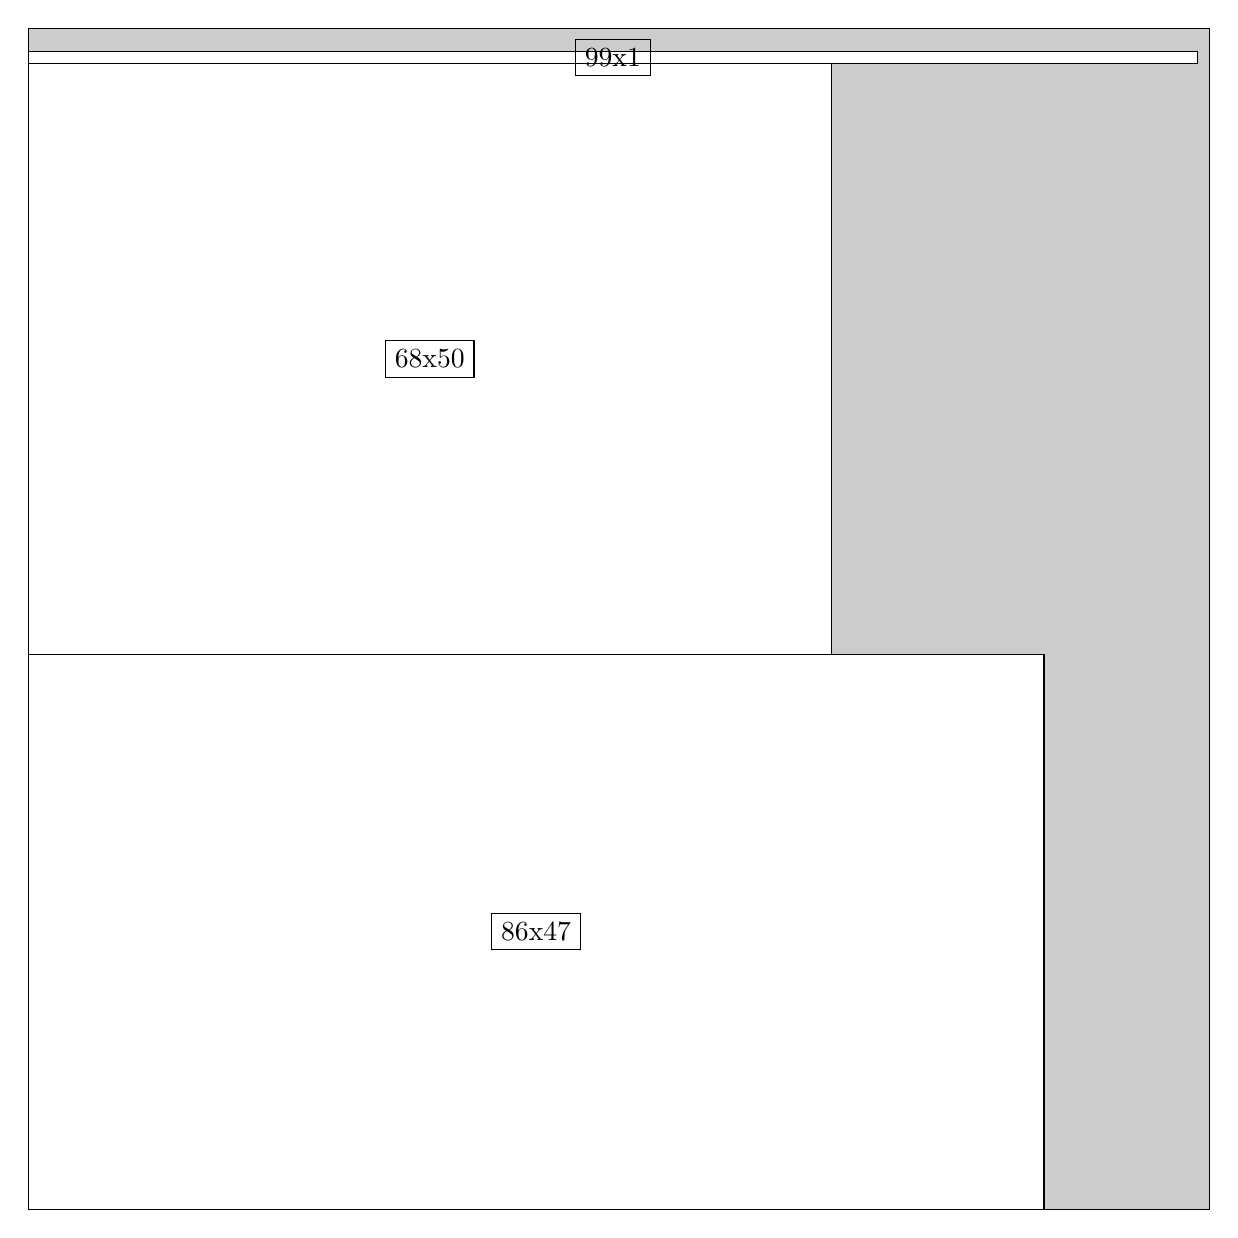
\begin{tikzpicture}[shorten >=1pt,scale=1.0,every node/.style={scale=1.0},->]
\tikzstyle{vertex}=[circle,fill=black!25,minimum size=14pt,inner sep=0pt]
\filldraw[fill=gray!40!white, draw=black] (0,0) rectangle (15.0,15.0);
\foreach \name/\x/\y/\w/\h in {86x47/0.0/0.0/12.9/7.05,68x50/0.0/7.05/10.2/7.5,99x1/0.0/14.549999999999999/14.85/0.15}
\filldraw[fill=white!40!white, draw=black] (\x,\y) rectangle node[draw] (\name) {\name} ++(\w,\h);
\end{tikzpicture}


w =86 , h =47 , x =0 , y =0 , v =4042
\par
w =68 , h =50 , x =0 , y =47 , v =3400
\par
w =99 , h =1 , x =0 , y =97 , v =99
\par
\newpage


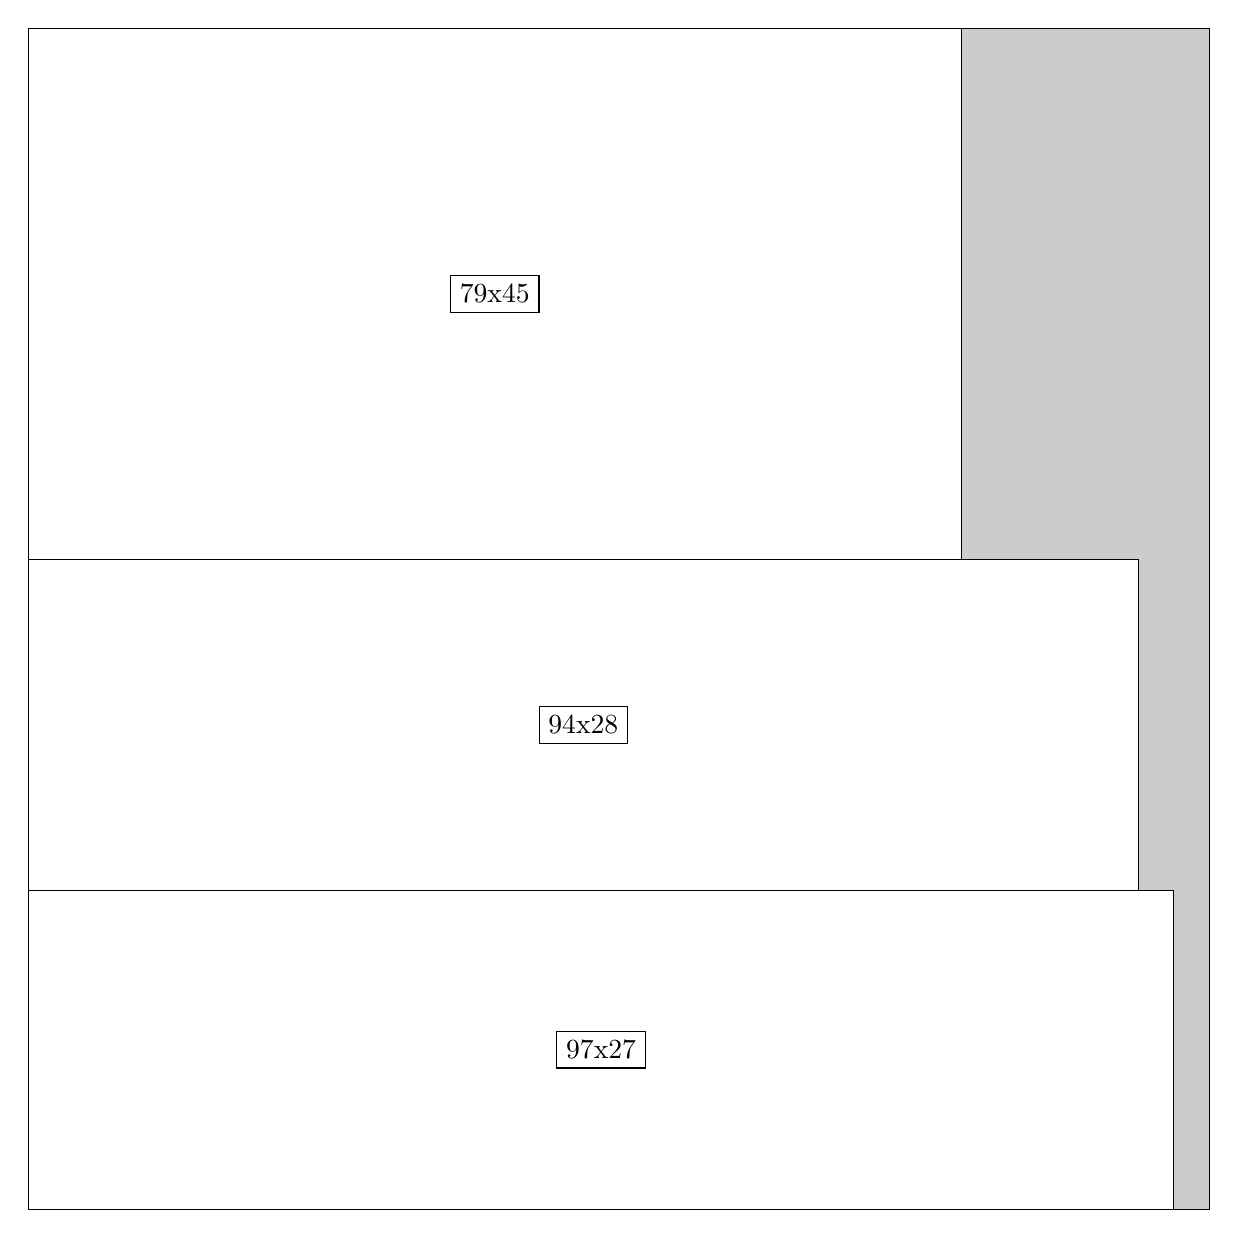
\begin{tikzpicture}[shorten >=1pt,scale=1.0,every node/.style={scale=1.0},->]
\tikzstyle{vertex}=[circle,fill=black!25,minimum size=14pt,inner sep=0pt]
\filldraw[fill=gray!40!white, draw=black] (0,0) rectangle (15.0,15.0);
\foreach \name/\x/\y/\w/\h in {79x45/0.0/8.25/11.85/6.75,94x28/0.0/4.05/14.1/4.2,97x27/0.0/0.0/14.549999999999999/4.05}
\filldraw[fill=white!40!white, draw=black] (\x,\y) rectangle node[draw] (\name) {\name} ++(\w,\h);
\end{tikzpicture}


w =79 , h =45 , x =0 , y =55 , v =3555
\par
w =94 , h =28 , x =0 , y =27 , v =2632
\par
w =97 , h =27 , x =0 , y =0 , v =2619
\par
\newpage


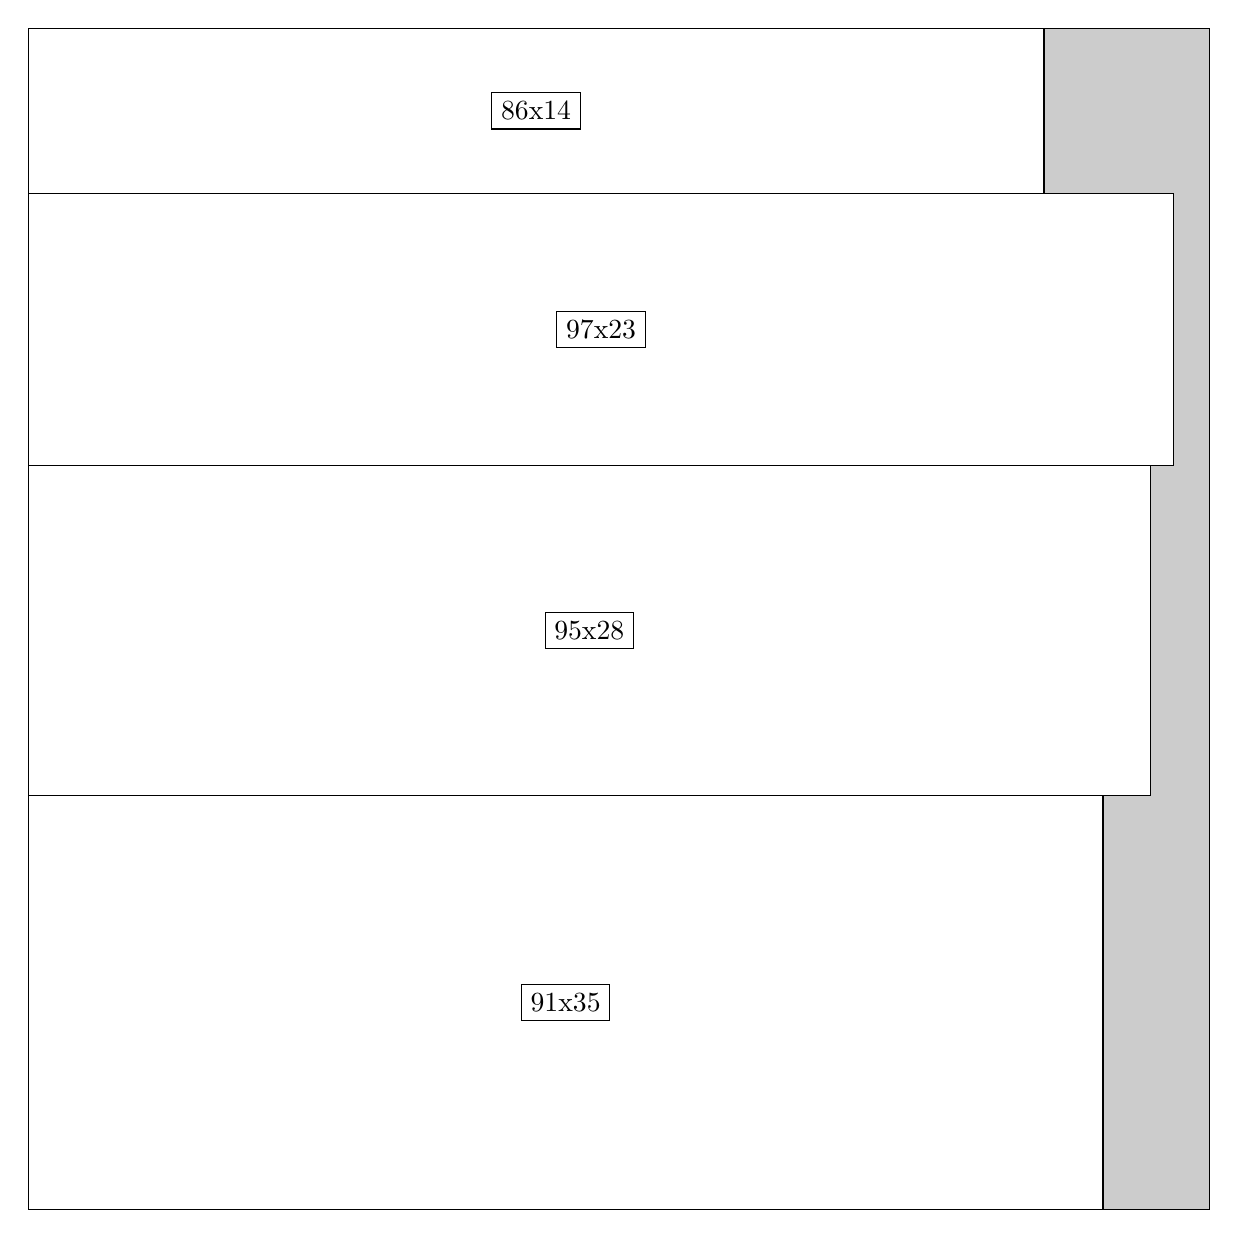
\begin{tikzpicture}[shorten >=1pt,scale=1.0,every node/.style={scale=1.0},->]
\tikzstyle{vertex}=[circle,fill=black!25,minimum size=14pt,inner sep=0pt]
\filldraw[fill=gray!40!white, draw=black] (0,0) rectangle (15.0,15.0);
\foreach \name/\x/\y/\w/\h in {91x35/0.0/0.0/13.65/5.25,95x28/0.0/5.25/14.25/4.2,97x23/0.0/9.45/14.549999999999999/3.4499999999999997,86x14/0.0/12.9/12.9/2.1}
\filldraw[fill=white!40!white, draw=black] (\x,\y) rectangle node[draw] (\name) {\name} ++(\w,\h);
\end{tikzpicture}


w =91 , h =35 , x =0 , y =0 , v =3185
\par
w =95 , h =28 , x =0 , y =35 , v =2660
\par
w =97 , h =23 , x =0 , y =63 , v =2231
\par
w =86 , h =14 , x =0 , y =86 , v =1204
\par
\newpage


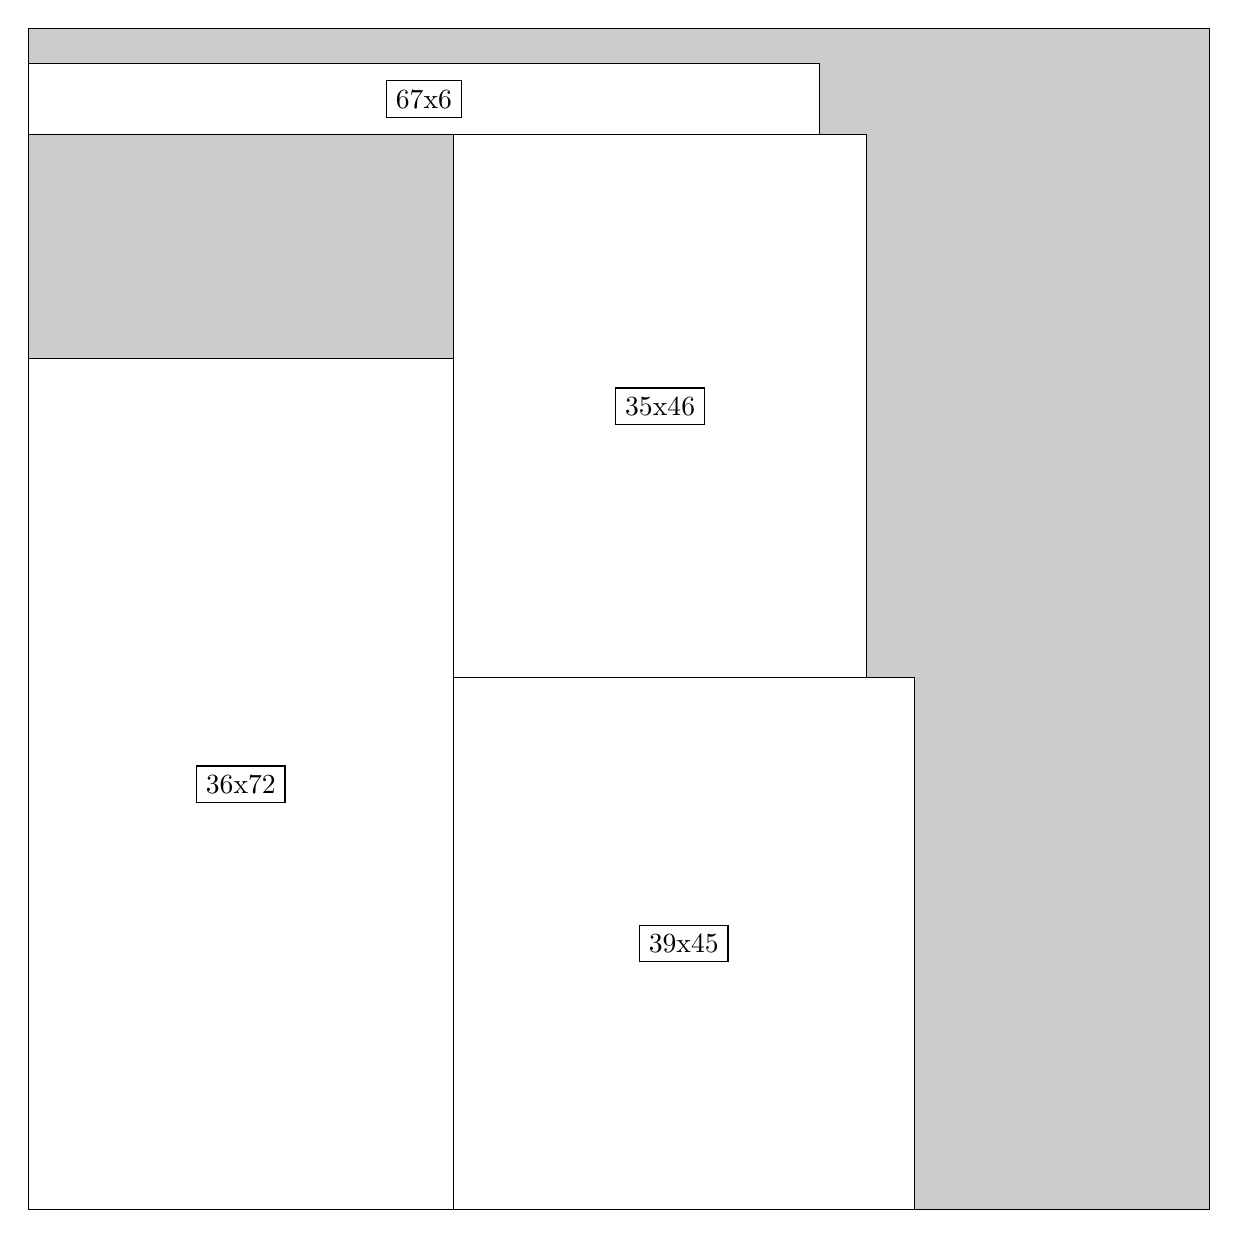
\begin{tikzpicture}[shorten >=1pt,scale=1.0,every node/.style={scale=1.0},->]
\tikzstyle{vertex}=[circle,fill=black!25,minimum size=14pt,inner sep=0pt]
\filldraw[fill=gray!40!white, draw=black] (0,0) rectangle (15.0,15.0);
\foreach \name/\x/\y/\w/\h in {36x72/0.0/0.0/5.3999999999999995/10.799999999999999,39x45/5.3999999999999995/0.0/5.85/6.75,35x46/5.3999999999999995/6.75/5.25/6.8999999999999995,67x6/0.0/13.65/10.049999999999999/0.8999999999999999}
\filldraw[fill=white!40!white, draw=black] (\x,\y) rectangle node[draw] (\name) {\name} ++(\w,\h);
\end{tikzpicture}


w =36 , h =72 , x =0 , y =0 , v =2592
\par
w =39 , h =45 , x =36 , y =0 , v =1755
\par
w =35 , h =46 , x =36 , y =45 , v =1610
\par
w =67 , h =6 , x =0 , y =91 , v =402
\par
\newpage


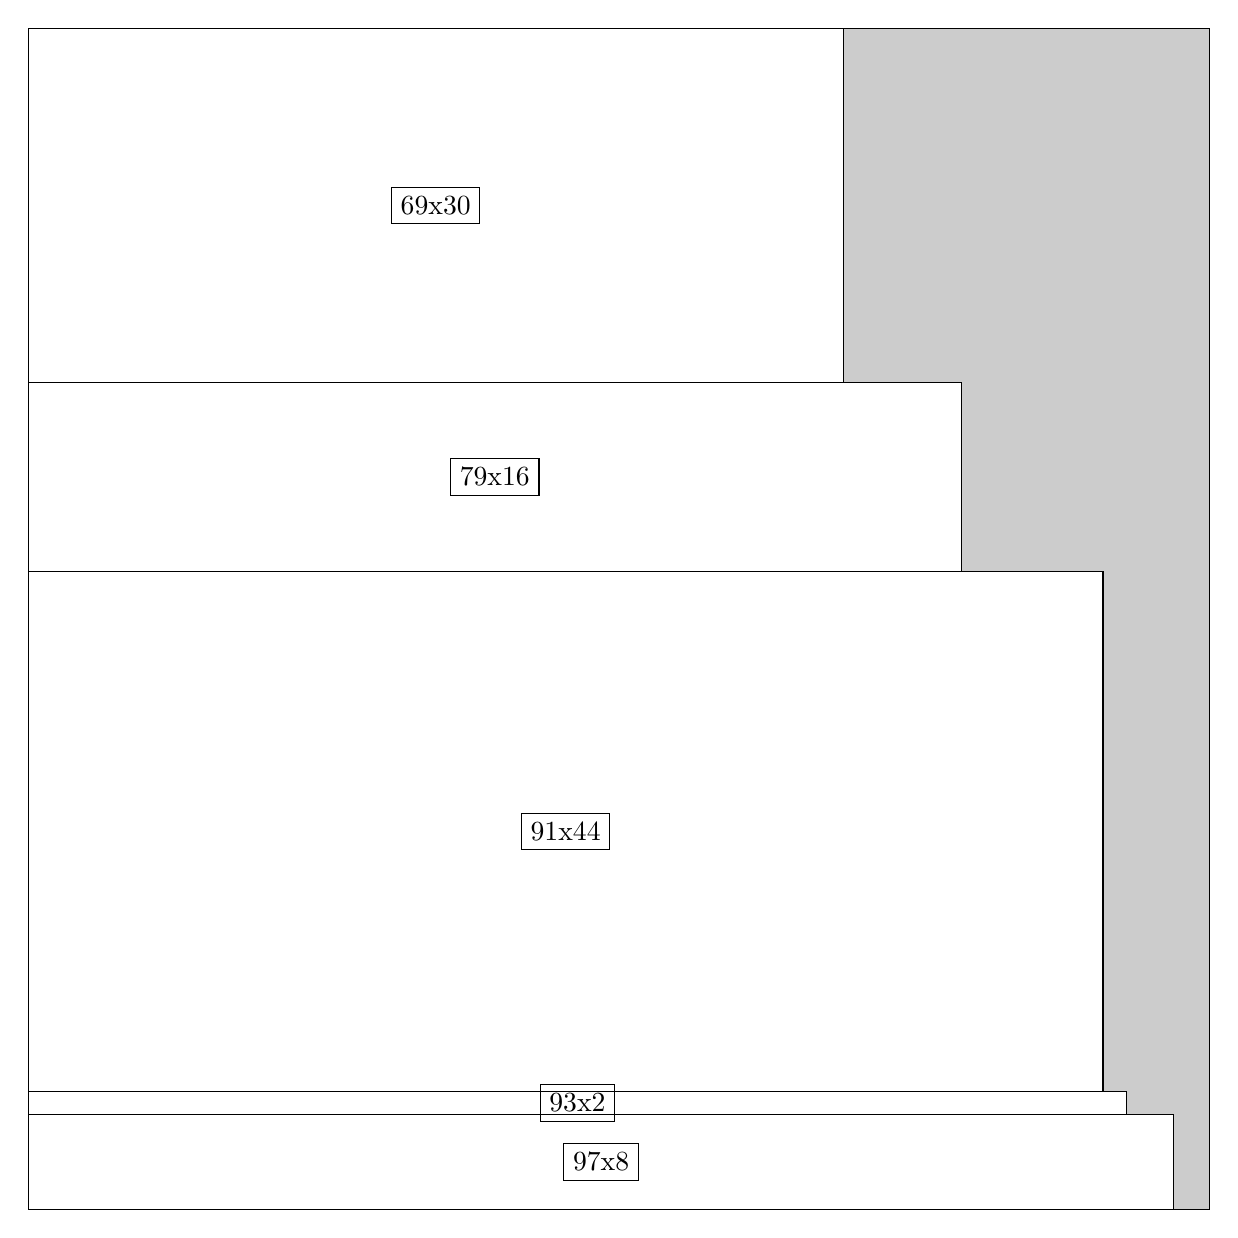
\begin{tikzpicture}[shorten >=1pt,scale=1.0,every node/.style={scale=1.0},->]
\tikzstyle{vertex}=[circle,fill=black!25,minimum size=14pt,inner sep=0pt]
\filldraw[fill=gray!40!white, draw=black] (0,0) rectangle (15.0,15.0);
\foreach \name/\x/\y/\w/\h in {91x44/0.0/1.5/13.65/6.6,69x30/0.0/10.5/10.35/4.5,79x16/0.0/8.1/11.85/2.4,97x8/0.0/0.0/14.549999999999999/1.2,93x2/0.0/1.2/13.95/0.3}
\filldraw[fill=white!40!white, draw=black] (\x,\y) rectangle node[draw] (\name) {\name} ++(\w,\h);
\end{tikzpicture}


w =91 , h =44 , x =0 , y =10 , v =4004
\par
w =69 , h =30 , x =0 , y =70 , v =2070
\par
w =79 , h =16 , x =0 , y =54 , v =1264
\par
w =97 , h =8 , x =0 , y =0 , v =776
\par
w =93 , h =2 , x =0 , y =8 , v =186
\par
\newpage


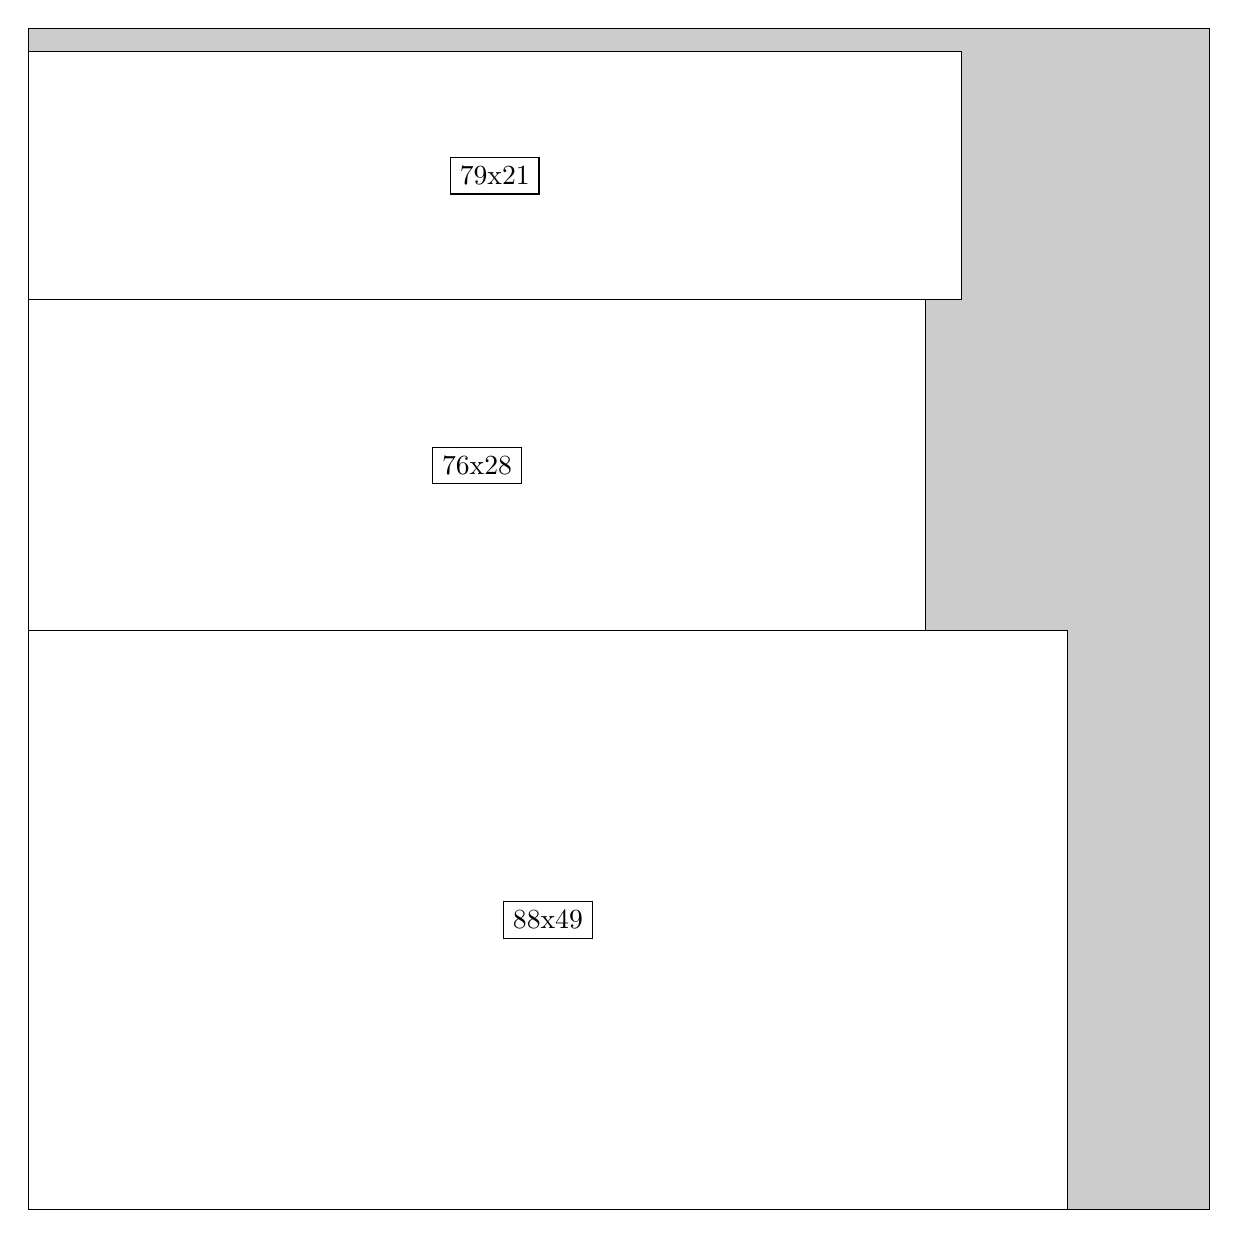
\begin{tikzpicture}[shorten >=1pt,scale=1.0,every node/.style={scale=1.0},->]
\tikzstyle{vertex}=[circle,fill=black!25,minimum size=14pt,inner sep=0pt]
\filldraw[fill=gray!40!white, draw=black] (0,0) rectangle (15.0,15.0);
\foreach \name/\x/\y/\w/\h in {88x49/0.0/0.0/13.2/7.35,76x28/0.0/7.35/11.4/4.2,79x21/0.0/11.549999999999999/11.85/3.15}
\filldraw[fill=white!40!white, draw=black] (\x,\y) rectangle node[draw] (\name) {\name} ++(\w,\h);
\end{tikzpicture}


w =88 , h =49 , x =0 , y =0 , v =4312
\par
w =76 , h =28 , x =0 , y =49 , v =2128
\par
w =79 , h =21 , x =0 , y =77 , v =1659
\par
\newpage


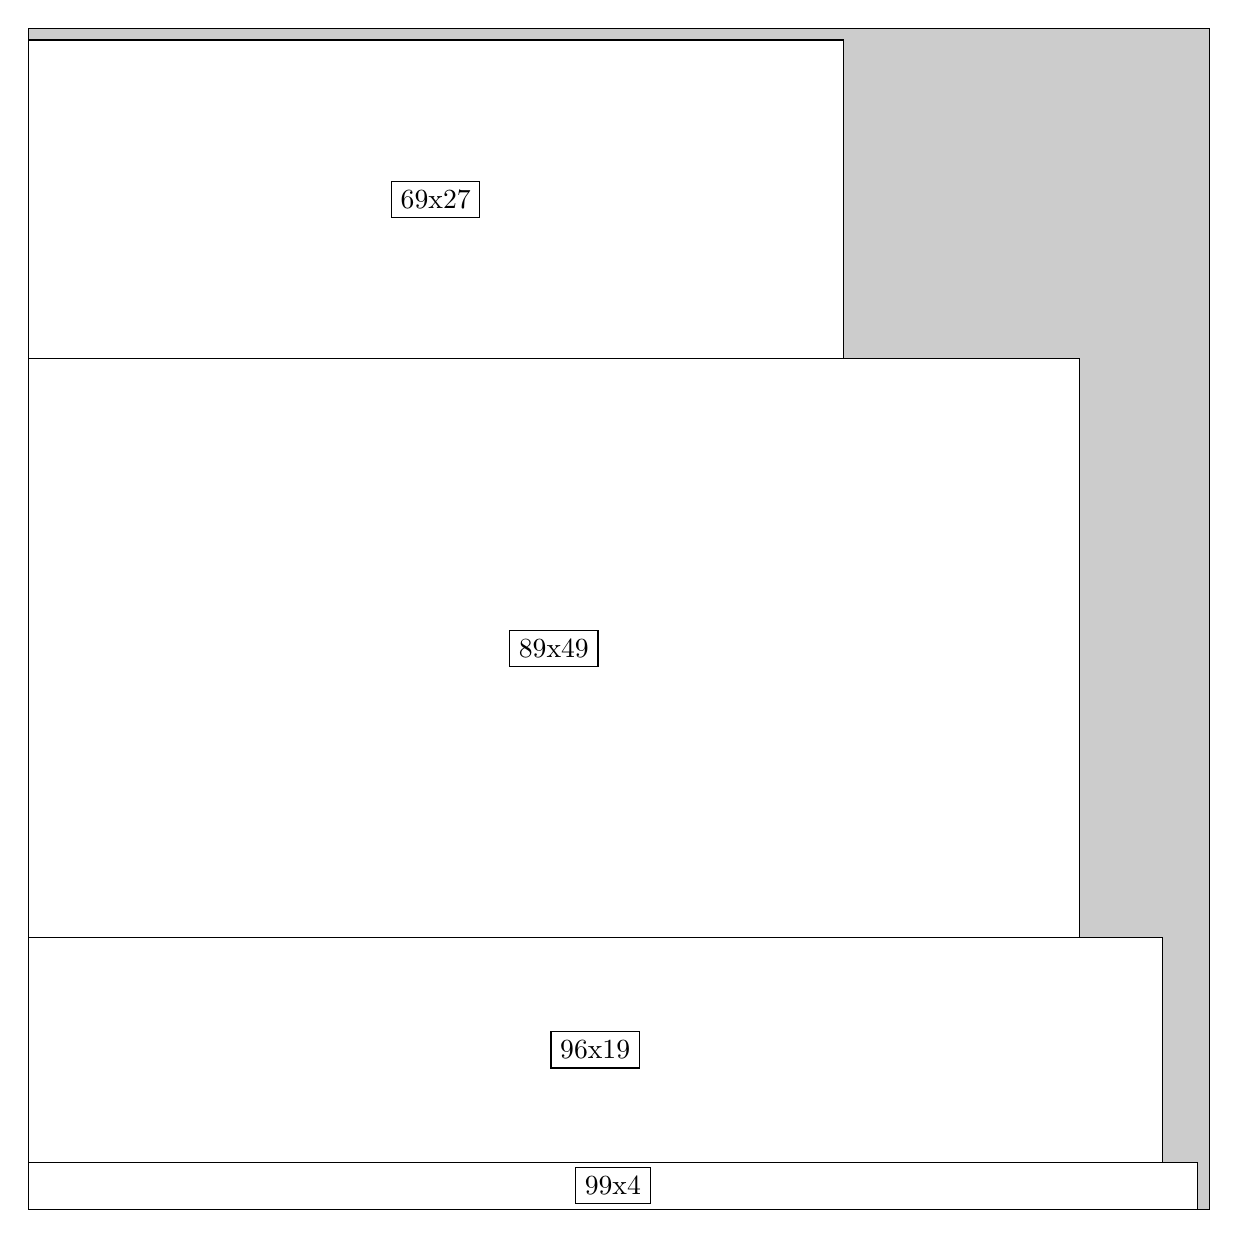
\begin{tikzpicture}[shorten >=1pt,scale=1.0,every node/.style={scale=1.0},->]
\tikzstyle{vertex}=[circle,fill=black!25,minimum size=14pt,inner sep=0pt]
\filldraw[fill=gray!40!white, draw=black] (0,0) rectangle (15.0,15.0);
\foreach \name/\x/\y/\w/\h in {89x49/0.0/3.4499999999999997/13.35/7.35,69x27/0.0/10.799999999999999/10.35/4.05,96x19/0.0/0.6/14.399999999999999/2.85,99x4/0.0/0.0/14.85/0.6}
\filldraw[fill=white!40!white, draw=black] (\x,\y) rectangle node[draw] (\name) {\name} ++(\w,\h);
\end{tikzpicture}


w =89 , h =49 , x =0 , y =23 , v =4361
\par
w =69 , h =27 , x =0 , y =72 , v =1863
\par
w =96 , h =19 , x =0 , y =4 , v =1824
\par
w =99 , h =4 , x =0 , y =0 , v =396
\par
\newpage


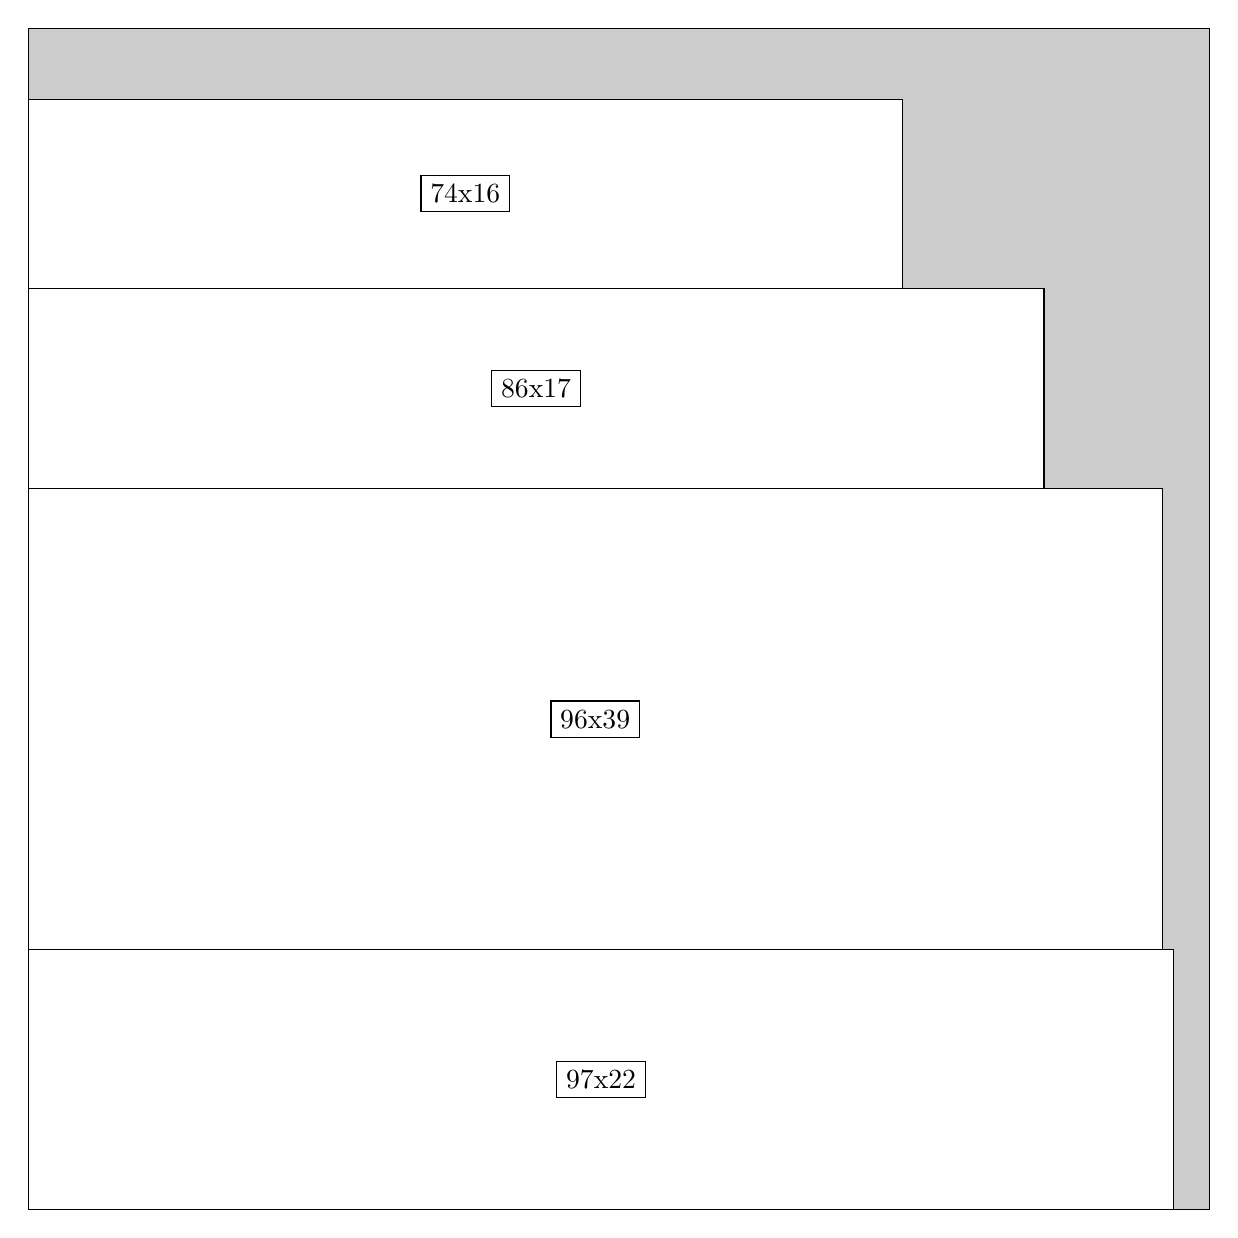
\begin{tikzpicture}[shorten >=1pt,scale=1.0,every node/.style={scale=1.0},->]
\tikzstyle{vertex}=[circle,fill=black!25,minimum size=14pt,inner sep=0pt]
\filldraw[fill=gray!40!white, draw=black] (0,0) rectangle (15.0,15.0);
\foreach \name/\x/\y/\w/\h in {74x16/0.0/11.7/11.1/2.4,97x22/0.0/0.0/14.549999999999999/3.3,86x17/0.0/9.15/12.9/2.55,96x39/0.0/3.3/14.399999999999999/5.85}
\filldraw[fill=white!40!white, draw=black] (\x,\y) rectangle node[draw] (\name) {\name} ++(\w,\h);
\end{tikzpicture}


w =74 , h =16 , x =0 , y =78 , v =1184
\par
w =97 , h =22 , x =0 , y =0 , v =2134
\par
w =86 , h =17 , x =0 , y =61 , v =1462
\par
w =96 , h =39 , x =0 , y =22 , v =3744
\par
\newpage


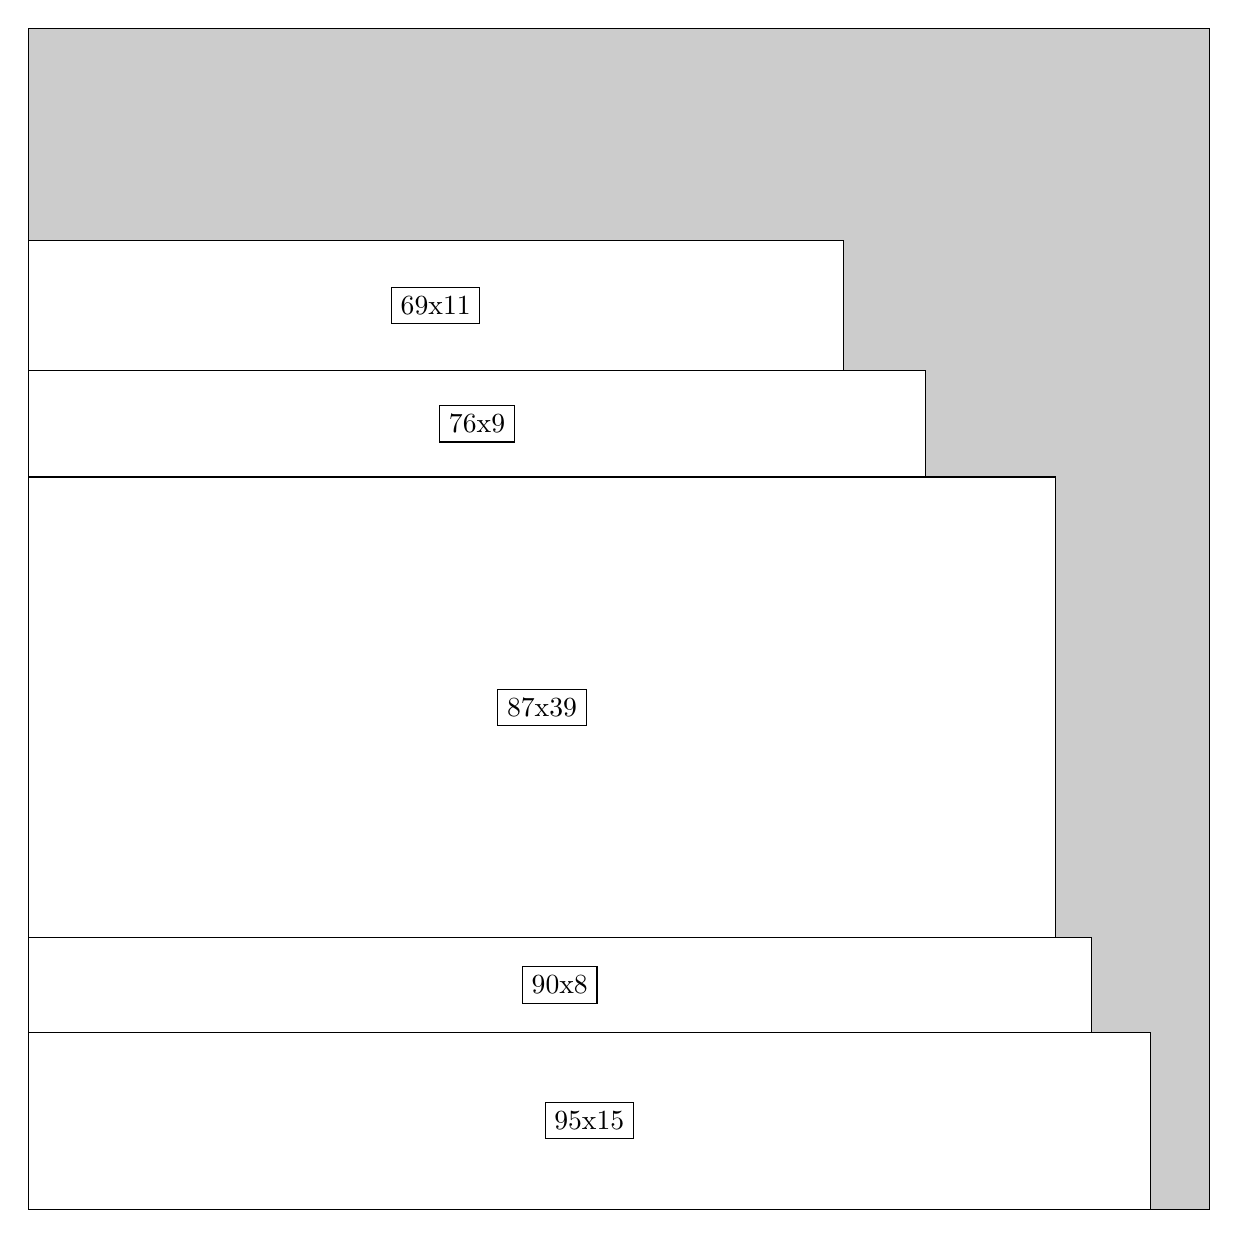
\begin{tikzpicture}[shorten >=1pt,scale=1.0,every node/.style={scale=1.0},->]
\tikzstyle{vertex}=[circle,fill=black!25,minimum size=14pt,inner sep=0pt]
\filldraw[fill=gray!40!white, draw=black] (0,0) rectangle (15.0,15.0);
\foreach \name/\x/\y/\w/\h in {87x39/0.0/3.4499999999999997/13.049999999999999/5.85,95x15/0.0/0.0/14.25/2.25,69x11/0.0/10.65/10.35/1.65,90x8/0.0/2.25/13.5/1.2,76x9/0.0/9.299999999999999/11.4/1.3499999999999999}
\filldraw[fill=white!40!white, draw=black] (\x,\y) rectangle node[draw] (\name) {\name} ++(\w,\h);
\end{tikzpicture}


w =87 , h =39 , x =0 , y =23 , v =3393
\par
w =95 , h =15 , x =0 , y =0 , v =1425
\par
w =69 , h =11 , x =0 , y =71 , v =759
\par
w =90 , h =8 , x =0 , y =15 , v =720
\par
w =76 , h =9 , x =0 , y =62 , v =684
\par
\newpage


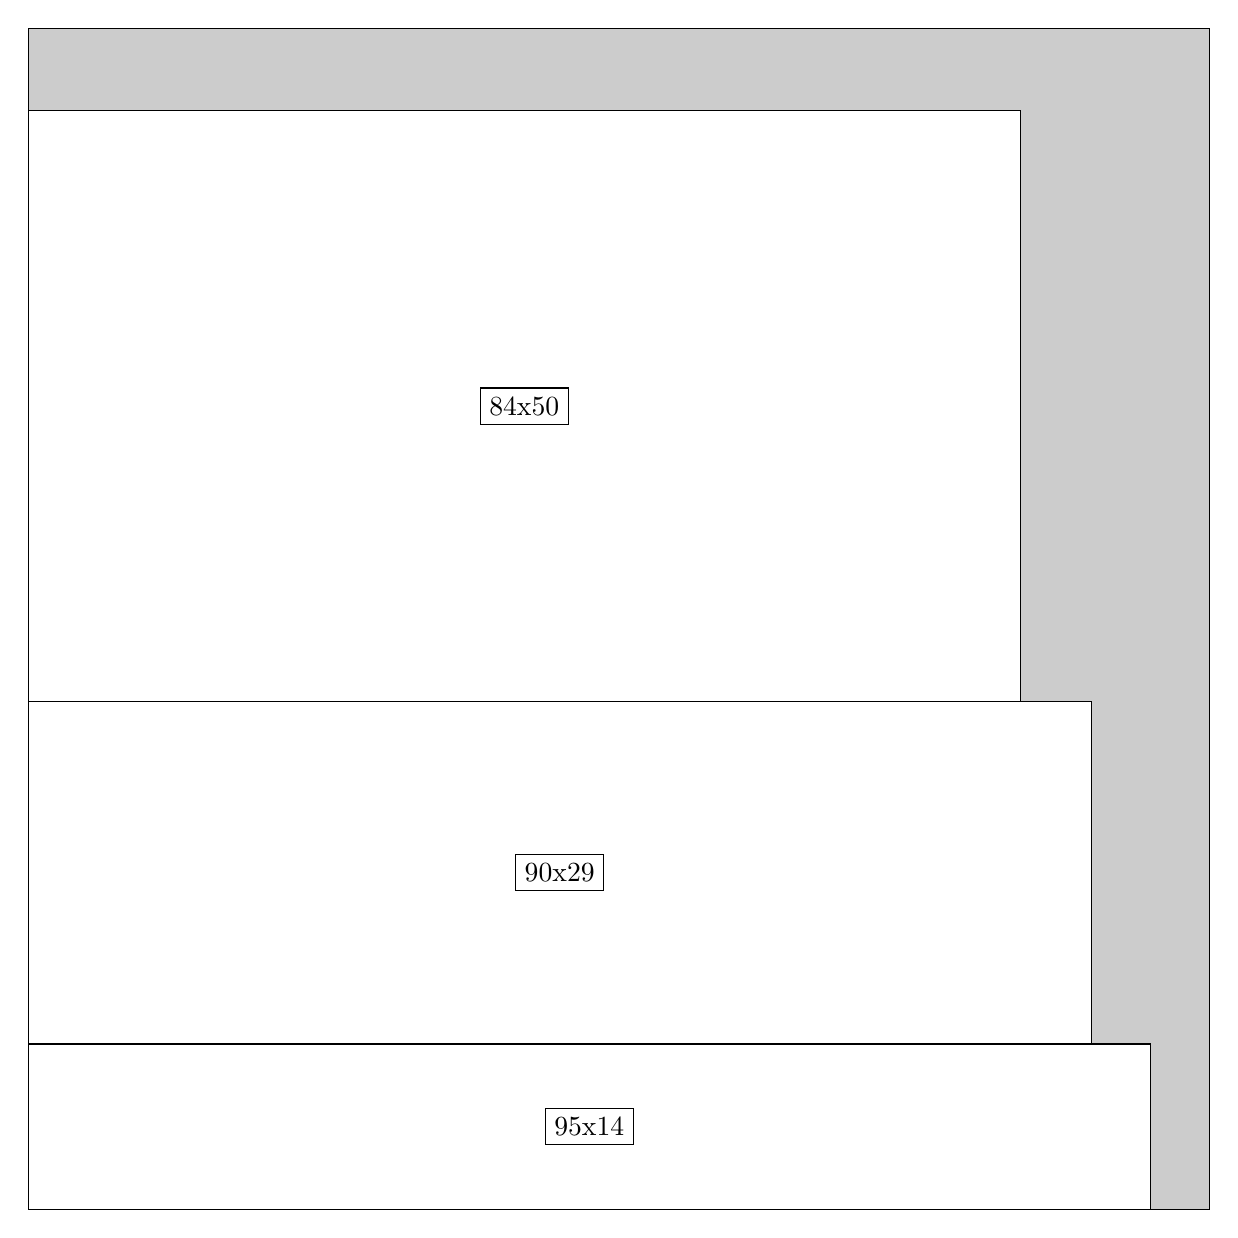
\begin{tikzpicture}[shorten >=1pt,scale=1.0,every node/.style={scale=1.0},->]
\tikzstyle{vertex}=[circle,fill=black!25,minimum size=14pt,inner sep=0pt]
\filldraw[fill=gray!40!white, draw=black] (0,0) rectangle (15.0,15.0);
\foreach \name/\x/\y/\w/\h in {84x50/0.0/6.45/12.6/7.5,90x29/0.0/2.1/13.5/4.35,95x14/0.0/0.0/14.25/2.1}
\filldraw[fill=white!40!white, draw=black] (\x,\y) rectangle node[draw] (\name) {\name} ++(\w,\h);
\end{tikzpicture}


w =84 , h =50 , x =0 , y =43 , v =4200
\par
w =90 , h =29 , x =0 , y =14 , v =2610
\par
w =95 , h =14 , x =0 , y =0 , v =1330
\par
\newpage


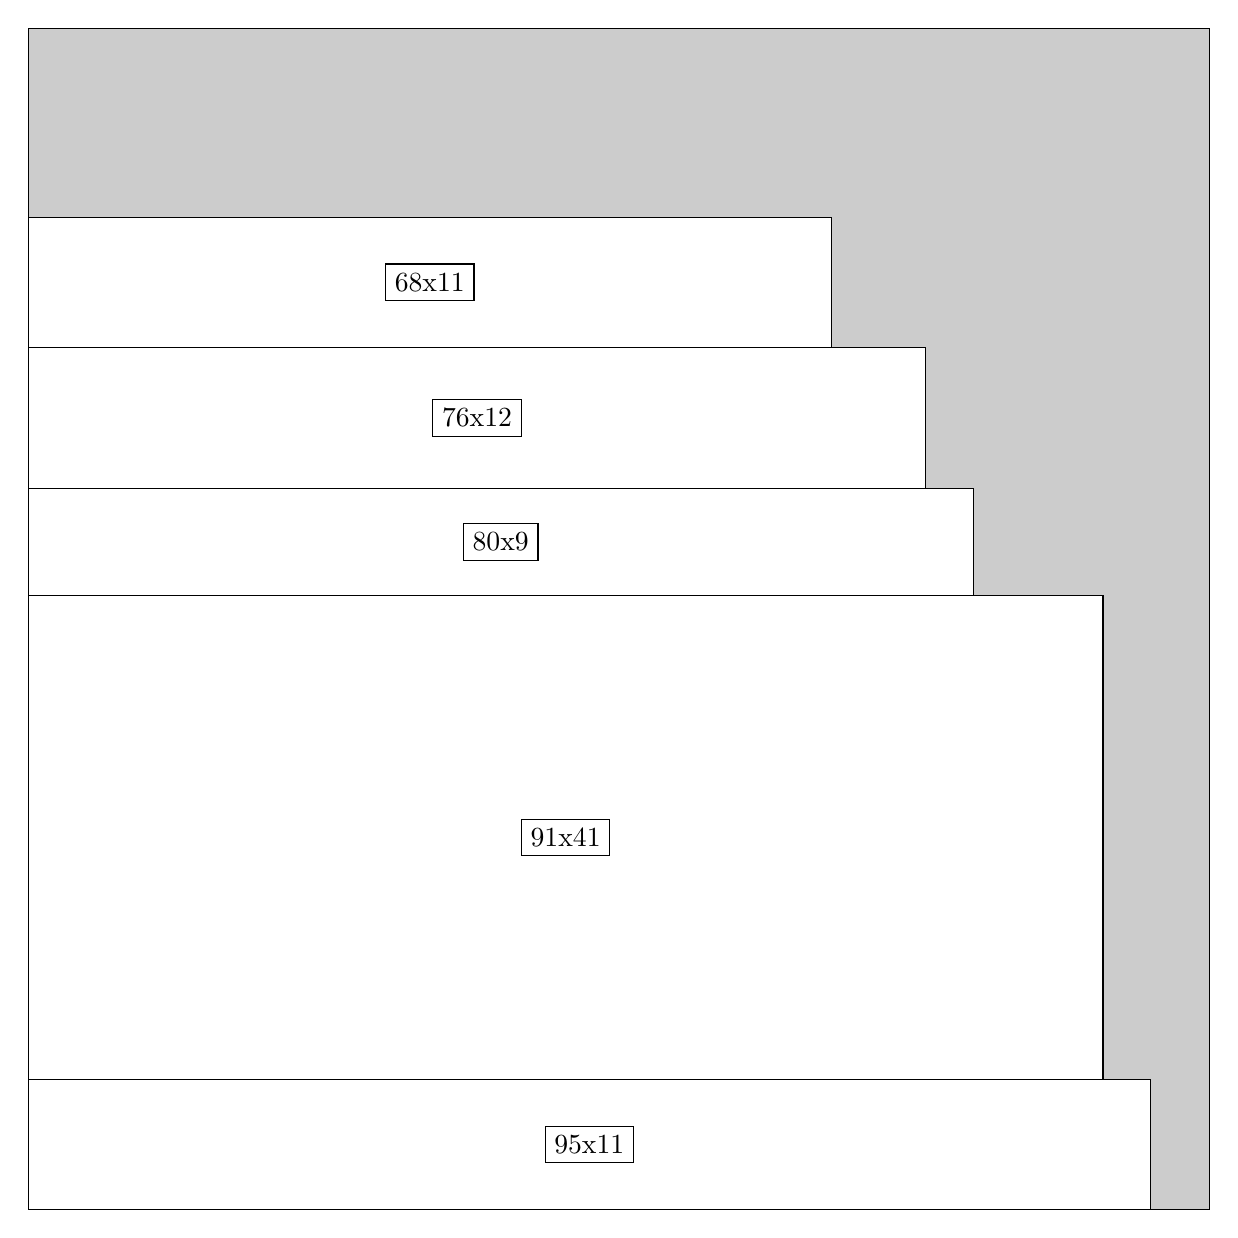
\begin{tikzpicture}[shorten >=1pt,scale=1.0,every node/.style={scale=1.0},->]
\tikzstyle{vertex}=[circle,fill=black!25,minimum size=14pt,inner sep=0pt]
\filldraw[fill=gray!40!white, draw=black] (0,0) rectangle (15.0,15.0);
\foreach \name/\x/\y/\w/\h in {91x41/0.0/1.65/13.65/6.1499999999999995,95x11/0.0/0.0/14.25/1.65,76x12/0.0/9.15/11.4/1.7999999999999998,68x11/0.0/10.95/10.2/1.65,80x9/0.0/7.8/12.0/1.3499999999999999}
\filldraw[fill=white!40!white, draw=black] (\x,\y) rectangle node[draw] (\name) {\name} ++(\w,\h);
\end{tikzpicture}


w =91 , h =41 , x =0 , y =11 , v =3731
\par
w =95 , h =11 , x =0 , y =0 , v =1045
\par
w =76 , h =12 , x =0 , y =61 , v =912
\par
w =68 , h =11 , x =0 , y =73 , v =748
\par
w =80 , h =9 , x =0 , y =52 , v =720
\par
\newpage


\end{document}